\PassOptionsToPackage{unicode}{hyperref}
\documentclass[aspectratio=1610, captions=tableheading, 11pt]{beamer}
\usepackage{booktabs}
% Load packages you need here
\usepackage{polyglossia}
\setmainlanguage{german}

\usepackage{csquotes}

%% Macros for Quote

\def\signed #1{{\leavevmode\unskip\nobreak\hfil\penalty50\hskip1em
  \hbox{}\nobreak\hfill #1%
  \parfillskip=0pt \finalhyphendemerits=0 \endgraf}}

\newsavebox\mybox
\newenvironment{aquote}[1]
  {\savebox\mybox{#1}\begin{quote}}
  {\vspace*{5mm}\signed{\usebox\mybox}\end{quote}}
    
%% \Macros

\usepackage{appendixnumberbeamer} 

\usepackage{caption}
\usepackage{varwidth}
\DeclareCaptionFormat{myformat}{%
  % #1: label (e.g. "Table 1")
  % #2: separator (e.g. ": ")
  % #3: caption text
  \begin{varwidth}{\linewidth}%
    \centering
    #1#2#3%
  \end{varwidth}%
}

%\AtBeginSection[]{
%  \begin{frame}
%  \vfill
%  \centering
%  \begin{beamercolorbox}[sep=8pt,center,shadow=true,rounded=true]{title}
%    \usebeamerfont{title}\insertsectionhead\par%
%  \end{beamercolorbox}
%  \vfill
%  \end{frame}
%}

\usepackage{amsmath}
\usepackage{amssymb}
\usepackage{mathtools}
\usepackage[mathrm=sym]{unicode-math}
\usepackage{relsize}
\usepackage{listings}

\usepackage[
  locale=DE,                 % deutsche Einstellungen
  separate-uncertainty=true, % immer Fehler mit \pm
  per-mode=reciprocal,       % ^-1 für inverse Einheiten
  % alternativ:
  % per-mode=reciprocal, % m s^{-1}
  % decimal-marker=., % . statt , f�r Dezimalzahlen
]{siunitx}

\usepackage{hyperref}
\usepackage{bookmark}
\usepackage[utf8]{inputenc}

% load the theme after all packages

\usetheme[
  showtotalframes, % show total number of frames in the footline
]{tudo}

% Put settings here, like
\unimathsetup{
  math-style=ISO,
  bold-style=ISO,
  nabla=upright,
  partial=upright,
  mathrm=sym,
}

% Flow chart stuff

\usepackage{tikz-feynman}
\usepackage{xfrac}
\usepackage{tikz}
\usetikzlibrary{shapes,arrows}


\tikzstyle{block} = [rectangle, draw, thick, fill=tugreen!20, 
    text width=20em, text centered, minimum height=2em]

 \tikzstyle{blockH} = [rectangle, draw, thick, fill=tugreen, 
    text width=20em, text centered, minimum height=2em]

\tikzstyle{smallblock} = [rectangle, draw, thick, fill=tugreen!20, 
    text width=14em, text centered, minimum height=2em]
\tikzstyle{smallblockH} = [rectangle, draw, thick, fill=tugreen, 
    text width=14em, text centered, minimum height=2em]

\tikzstyle{line} = [draw, -latex']


% Pseudocode Algorithm

\usepackage[german,onelanguage]{algorithm2e} %for psuedo code


% Evaluate at command

\NewDocumentCommand{\evalat}{sO{\big}mm}{%
  \IfBooleanTF{#1}
   {\mleft. #3 \mright|_{#4}}
   {#3#2|_{#4}}%
}


\setbeamertemplate{caption}{\raggedright\insertcaption\par}

% nur wenn akkurat auf dem Rechner installiert ist:
\setsansfont{Akkurat Light Office}[
  BoldFont=Akkurat Office Bold,
]


\author[jean-marco.alameddine@udo.edu]{Jean-Marco Alameddine}
\title{Masterarbeit - Aktueller Stand}      
\date[15.11.2019]{15.11.2019}

\institute[%
  {
\includegraphics[height=0.9\headerheight]{e5b.pdf}}%
]{Technische Universität Dortmund}

\newcommand\CC{C\nolinebreak[4]\hspace{-.05em}\raisebox{.4ex}{\relsize{-3}{\textbf{++}}}\:}
\titlegraphic{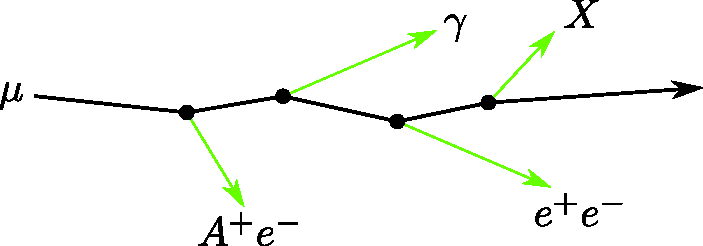
\includegraphics[height=0.5\textheight]{plots/muon_path.pdf}}

\usepackage{color}
\newcommand{\Hilight}{\makebox[0pt][l]{\color{tugreen}\rule[-4pt]{0.65\linewidth}{14pt}}}

\begin{document}



%%% TITLE

\begin{frame}
  \maketitle
\end{frame}

%%% Content

\begin{frame}[noframenumbering]{Inhalt}
   \begin{columns}
       \begin{column}{0.4\textwidth}

            \setbeamercolor{block title}{fg=white, bg=tugreen}
            \setbeamercolor{block body}{fg=darkgray, bg=tulight}

            \begin{block}{1. Einführung in PROPOSAL}
              \centering
                \vspace{2mm}
              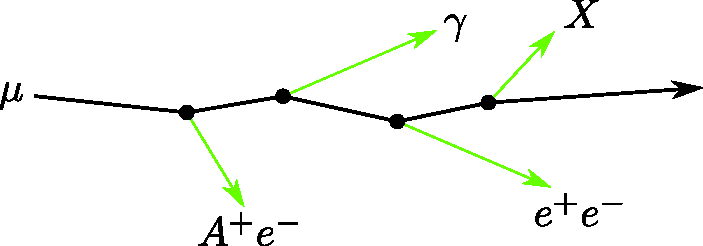
\includegraphics[height=0.15\textheight]{plots/muon_path.pdf}
                \vspace{2mm}
            \end{block}
       \end{column}
       \begin{column}{0.4\textwidth}

            \setbeamercolor{block title}{fg=white, bg=tugreen}
            \setbeamercolor{block body}{fg=darkgray, bg=tulight}

            \begin{block}{2. Seltene Prozesse}
            \centering
            \vspace{2mm}
			\resizebox{!}{0.15\textheight}{%
      			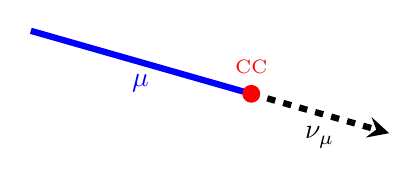
\begin{tikzpicture}
      				\centering
      							
	  				\draw [line width=0.8mm, blue] (-1.9, 1.8) -- node[below] {$\mu$}  (0.9, 1.);			
	  				\draw [line width=0.8mm, black, dashed, ->, >=stealth] (0.9, 1.) -- node[below] {$\nu_{\mu}$}  (0.9+1.4+0.35, 1. - 0.4 - 0.1);			
	  				\draw[red,fill=red] (0.9, 1.) circle (0.7ex) node[label=above: $\scriptsize \text{CC}$]{};
   				\end{tikzpicture}
   			}
   		\vspace{3mm}
            \end{block}

       \end{column}
   \end{columns}
   \begin{columns}
       \begin{column}{0.4\textwidth}

            \setbeamercolor{block title}{fg=white, bg=tugreen}
            \setbeamercolor{block body}{fg=darkgray, bg=tulight}

            \begin{block}{3. Schauerpropagation}
            \centering
            \vspace{2mm}
      \resizebox{!}{0.15\textheight}{%

            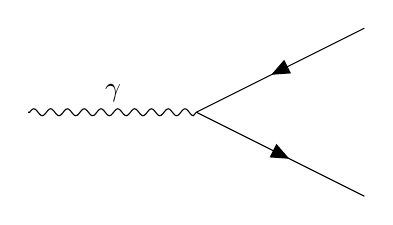
\begin{tikzpicture}
                  \centering
                   % Sizes
                   \pgfmathsetmacro{\len}{0.05cm}
                   \pgfmathsetmacro{\halflen}{\len/4}
                   \pgfmathsetmacro{\vertexsize}{\len/20}
                   \begin{feynman}
                       % vertices
                       \vertex (a) at (0, 0);
                       \vertex (b) at (1.5*\len, 0);
                       \vertex (c) at (3*\len, 0.75*\len);
                       \vertex (d) at (3*\len, -0.75*\len);;
                 
                       % draw diagram
                       \diagram* {
                         (c) -- [fermion] (b) -- [fermion] (d),
                         (a) -- [boson, edge label=\(\gamma\)] (b),
                       };   
                  \end{feynman}
            \end{tikzpicture}
            }
            \vspace{2.5mm}
           \end{block}
       \end{column}
       \begin{column}{0.4\textwidth}

            \setbeamercolor{block title}{fg=white, bg=tugreen}
            \setbeamercolor{block body}{fg=darkgray, bg=tulight}

           \begin{block}{4. Ergebnisse}
              \centering
                \vspace{2mm}
              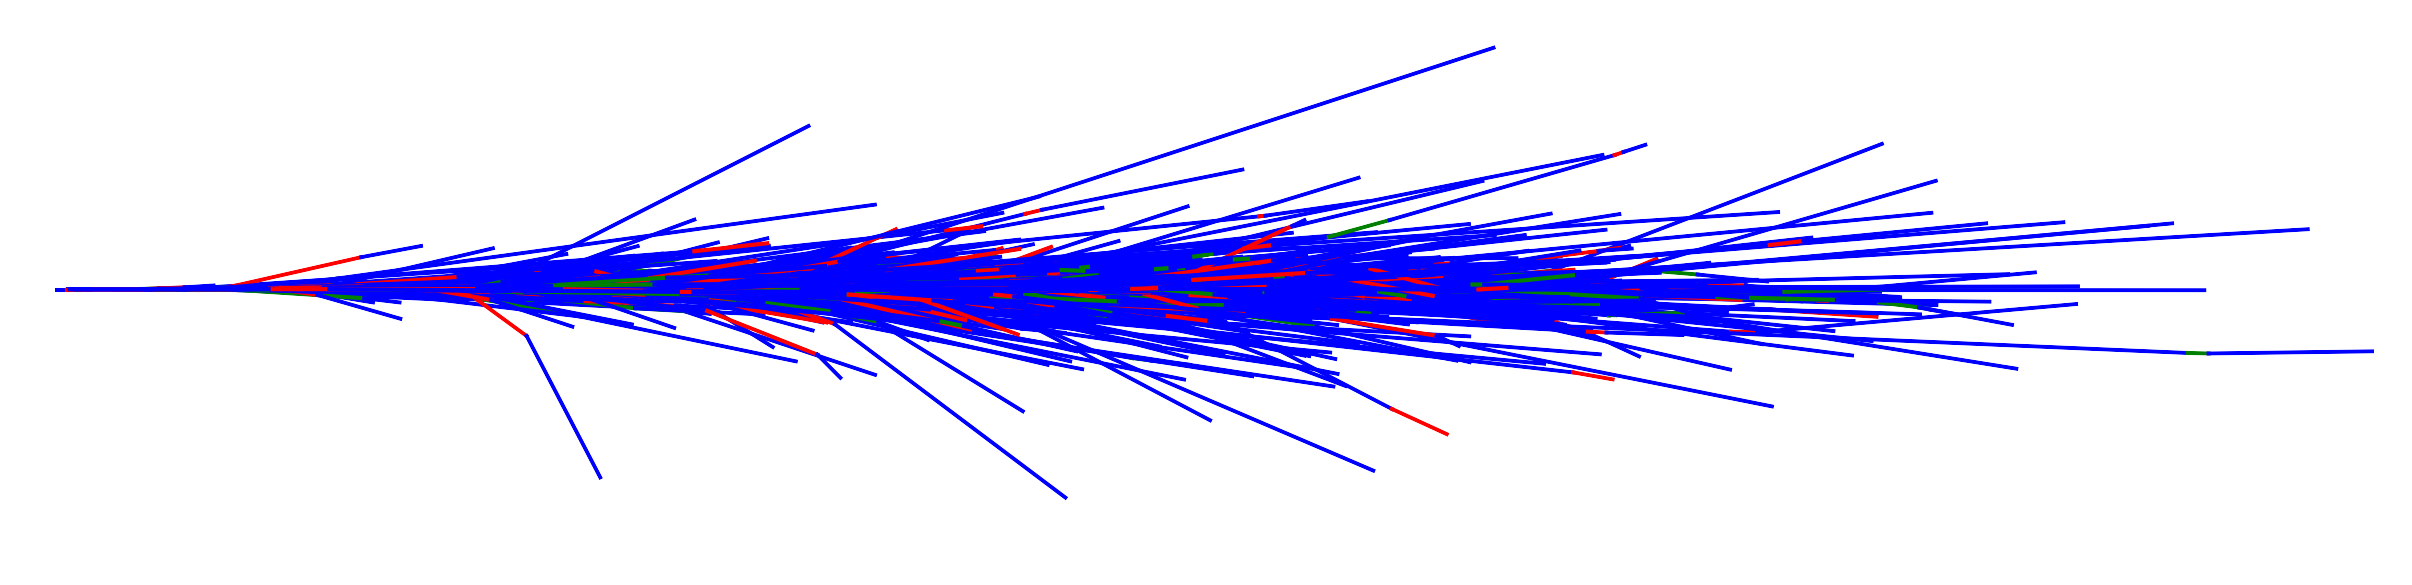
\includegraphics[height=0.15\textheight]{plots/shower_nolegend.png}
                \vspace{2mm}
           \end{block}
       \end{column}
   \end{columns}
\end{frame}

%%% 1. Einführung in PROPOSAL

% Contents slide

\begin{frame}[noframenumbering]{Inhalt}
   \begin{columns}
       \begin{column}{0.4\textwidth}

            \setbeamercolor{block title}{fg=white, bg=tugreen}
            \setbeamercolor{block body}{fg=darkgray, bg=tulight}

            \begin{block}{1. Einführung in PROPOSAL}
              \centering
                \vspace{2mm}
              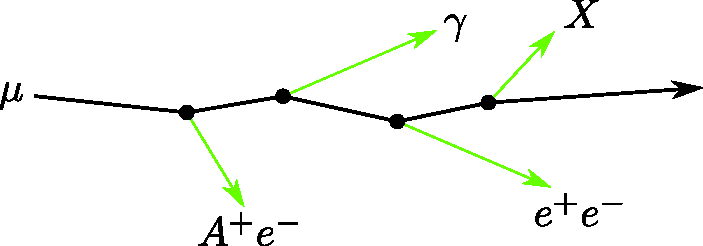
\includegraphics[height=0.15\textheight]{plots/muon_path.pdf}
                \vspace{2mm}
            \end{block}
       \end{column}
       \begin{column}{0.4\textwidth}

            \setbeamercolor{block title}{fg=white, bg=darkgray}
            \setbeamercolor{block body}{fg=darkgray, bg=gray}

            \begin{block}{2. Seltene Prozesse}
            \centering
            \vspace{2mm}
      \resizebox{!}{0.15\textheight}{%
            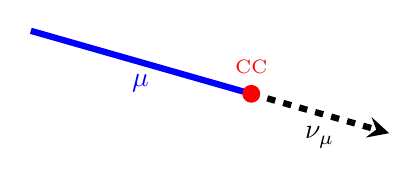
\begin{tikzpicture}
              \centering
                    
            \draw [line width=0.8mm, blue] (-1.9, 1.8) -- node[below] {$\mu$}  (0.9, 1.);     
            \draw [line width=0.8mm, black, dashed, ->, >=stealth] (0.9, 1.) -- node[below] {$\nu_{\mu}$}  (0.9+1.4+0.35, 1. - 0.4 - 0.1);      
            \draw[red,fill=red] (0.9, 1.) circle (0.7ex) node[label=above: $\scriptsize \text{CC}$]{};
          \end{tikzpicture}
        }
      \vspace{3mm}
            \end{block}

       \end{column}
   \end{columns}
   \begin{columns}
       \begin{column}{0.4\textwidth}

            \setbeamercolor{block title}{fg=white, bg=darkgray}
            \setbeamercolor{block body}{fg=darkgray, bg=gray}

          \begin{block}{3. Schauerpropagation}
            \centering
            \vspace{2mm}
            \resizebox{!}{0.15\textheight}{%

            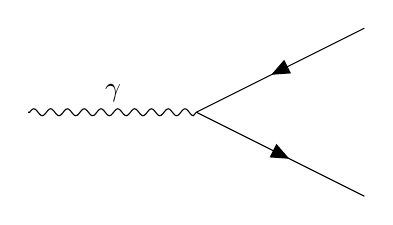
\begin{tikzpicture}
                  \centering
                   % Sizes
                   \pgfmathsetmacro{\len}{0.05cm}
                   \pgfmathsetmacro{\halflen}{\len/4}
                   \pgfmathsetmacro{\vertexsize}{\len/20}
                   \begin{feynman}
                       % vertices
                       \vertex (a) at (0, 0);
                       \vertex (b) at (1.5*\len, 0);
                       \vertex (c) at (3*\len, 0.75*\len);
                       \vertex (d) at (3*\len, -0.75*\len);;
                 
                       % draw diagram
                       \diagram* {
                         (c) -- [fermion] (b) -- [fermion] (d),
                         (a) -- [boson, edge label=\(\gamma\)] (b),
                       };   
                  \end{feynman}
            \end{tikzpicture}
            }
            \vspace{2.5mm}
           \end{block}
       \end{column}
       \begin{column}{0.4\textwidth}

            \setbeamercolor{block title}{fg=white, bg=darkgray}
            \setbeamercolor{block body}{fg=darkgray, bg=gray}

           \begin{block}{4. Ergebnisse}
              \centering
                \vspace{2mm}
              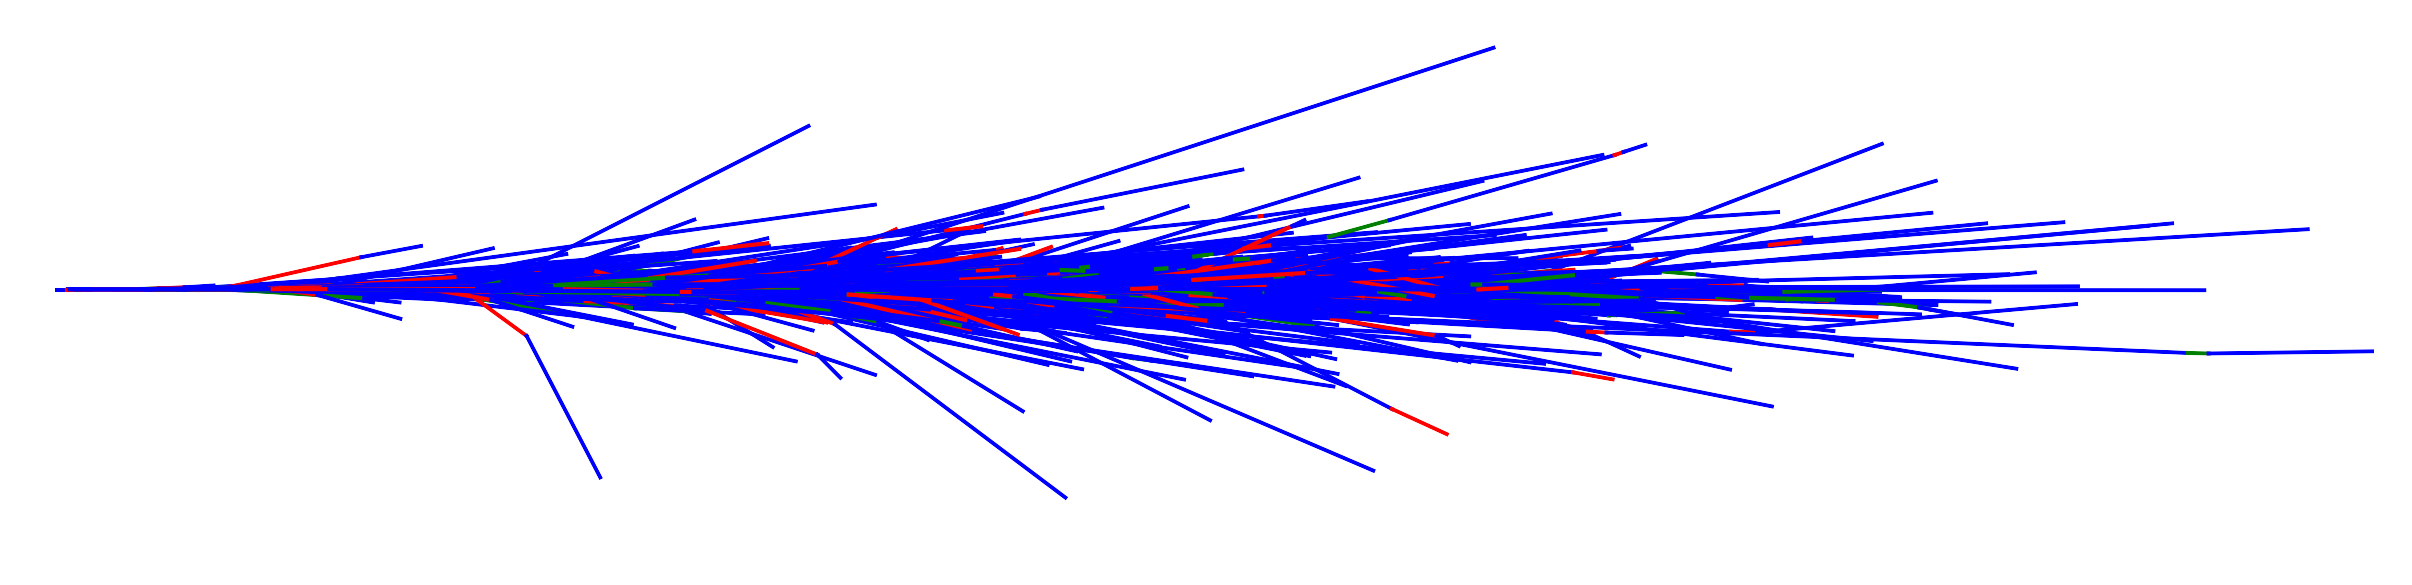
\includegraphics[height=0.15\textheight]{plots/shower_nolegend.png}
                \vspace{2mm}
           \end{block}
       \end{column}
   \end{columns}
\end{frame}

\section{Einführung in PROPOSAL - Motivation}

\begin{frame}
      \begin{aquote}{"Der Leptonpropagator PROPOSAL" - Dissertation von Jan-Hendrik Köhne}
      Ziel ist es ein Monte-Carlo Programm zu entwickeln, welches einerseits die bei der \textcolor{red}{Propagation von Leptonen} auftauchende große Anzahl an Wechselwirkungen (einige tausend)
      mit \textcolor{red}{großer Genauigkeit} beschreibt und andererseits den \textcolor{red}{algorithmischen Fehler} so gering wie möglich hält. 
      \end{aquote}
\end{frame}

\begin{frame}
  \begin{columns}
    \column{0.62\textwidth}
    \begin{center}
      \begin{itemize}
        \setlength\itemsep{0.5em}
        \item \textbf{PROPOSAL}: \CC-Bibliothek mit Python Bindings
        \item Simulation der physikalischen Wechselwirkungen hochenergetischer Teilchen
        \begin{itemize}
          \item[$\rightarrow$] Energieverluste durch Interaktionen
          \item[$\rightarrow$] Vielfachstreuung
          \item[$\rightarrow$] Zerfall am Ende der Lebensdauer
        \end{itemize}
        \item Verschiedene Parametrisierungen für die physikalischen Wechselwirkungen verfügbar
        \begin{itemize}
          \item[$\rightarrow$] Untersuche Auswirkungen auf Simulationen
        \end{itemize}
      \end{itemize}
  \end{center}
  \column{0.35\textwidth}
      \begin{figure}
          \centering
          
\includegraphics[width=0.8\linewidth]{plots/github.pdf}
           \captionsetup{format=myformat}
          \caption*{https://github.com/tudo-astroparticlephysics/PROPOSAL}
      \end{figure}
  \end{columns}

\end{frame}

\section{Einführung in PROPOSAL - Algorithmus}

\begin{frame}
  \Huge
  \begin{align*}
      \frac{\mathrm{d}\sigma}{\mathrm{d}v} \quad \underbrace{\longrightarrow}_{?} \quad \text{Energieverluste}
  \end{align*}\\[1cm]
  \large
  \centering
  mit $v$ dem relativen Energieverlust eines Primärteilchens
\end{frame}

\begin{frame}
  \huge
  \begin{align*}
      \underset{\text{stochastische Verluste}}{v > v_\text{cut}} &&  \underset{\text{kontinuierliche Verluste}}{v < v_\text{cut}}
  \end{align*}\\
  \vspace{20px}
    \Large
    \centering
  mit $v_\text{cut} = \text{min}\left[\sfrac{e_\text{cut}}{E}, v\prime_\text{cut} \right]$
\end{frame}


\begin{frame}[fragile]
  \begin{columns}
    \column{0.55\textwidth}
    \begin{center}
        \begin{tikzpicture}[node distance = 1.2cm, auto]
          % Place nodes
          \footnotesize

          \node [smallblock] (zero) {Startenergie $E_i$};
          \onslide<1>{\node [smallblockH] (zero) {Startenergie $E_i$};}

          \node [block, below of=zero] (one) {Würfle Energie $E_f$ bei welcher der nächste stoch. Verlust auftritt};
          \onslide<2>{\node [blockH, below of=zero] (one) {Würfle Energie $E_f$ bei welcher der nächste stoch. Verlust auftritt};}
      
          \node [block, below of=one] (two) {Berechne Strecke bis zum nächsten stoch. Verlust};
          \onslide<3>{\node [blockH, below of=one] (two) {Berechnte Strecke bis zum nächsten stoch. Verlust};}
      
          \node [block, below of=two] (three) {Würfle Art des stoch. Verlustes};
          \onslide<4>{\node [blockH, below of=two] (three) {Würfle Art des stoch. Verlustes};}
      
          \node [block, below of=three] (four) {Würfle Größe des stoch. Verlustes};
          \onslide<5>{\node [blockH, below of=three] (four) {Würfle Größe des stoch. Verlustes};}

          \node [block, below of=four] (five) {Wiederhole bis $E < e_\text{low}$ oder Teilchen zerfallen};
          \onslide<6>{\node [blockH, below of=four] (five) {Wiederhole bis $E < e_\text{low}$ oder Teilchen zerfallen};}
      
          % Draw edges
          \path [line, ultra thick] (zero) -- (one);
          \path [line, ultra thick] (one) -- (two);
          \path [line, ultra thick] (two) -- (three);
          \path [line, ultra thick] (three) -- (four);
          \path [line, ultra thick] (four) -- (five);

          \onslide<6>
          { 
            \path [line, ultra thick] (five.east) -- +(1,0) |- node[pos=0.25] {} (one);
          }
        \end{tikzpicture}

  \end{center}

  \column{0.4\textwidth}
  \begin{overprint}
      \only<1>
      {      
          \centering
          \begin{block}{Initialisierung}
          Setze $E_i, \vec{r_i}, \vec{d_i}, \dots$ für zu propagierendes Teilchen
          \end{block}
      }

      \only<2>
      { 
        \centering
        \begin{block}{Energieintegral}
          \begin{align*}
            \int_{E_i}^{E_f} \frac{\sigma\left(E\right)}{-f\left(E\right)} \cdot \mathrm{d}E = -\log{\left( \xi \right)} 
          \end{align*}
          \begin{itemize}
            \item $\sigma\left(E\right) = \sigma_\text{\tiny tot, stoch}$ \\[0.25cm]
            \item $f\left(E\right) = \evalat{\frac{\mathrm{d}E}{\mathrm{d}x}}{\text{\tiny kont.}} \propto E \int_{v_\text{min}}^{v_\text{cut}} v \frac{\mathrm{d}\sigma}{\mathrm{d}v}\mathrm{d}v$  \\[0.25cm]
            \item $\xi \in \left[0, 1 \right)$
          \end{itemize}
        \end{block}
      }

      \only<3>
      { 
        \centering
        \begin{block}{Spurintegral}
          \begin{align*}
            x_f = x_i - \int_{E_i}^{E_f} \frac{\mathrm{d}E}{f\left(E\right)} 
          \end{align*}

          \begin{itemize}
            \item $f\left(E\right) = \evalat{\frac{\mathrm{d}E}{\mathrm{d}x}}{\text{\tiny kont.}} \propto E \int_{v_\text{min}}^{v_\text{cut}} v \frac{\mathrm{d}\sigma}{\mathrm{d}v}\mathrm{d}v$ 
          \end{itemize}        
        \end{block}
      }

      \only<4>
      { 
        \centering
        \begin{block}{Stochastischer Verlust}
          Vergleiche $\sigma_\text{tot, stoch}$ der verschiedenen Wechselwirkungen.\\
        \end{block}
      }

      \only<5>
      { 
        \centering
        \begin{block}{Stochastischer Verlust}
          \begin{align*}
              \frac{1}{\sigma_{i, \text{tot}}} \int_{v_\text{cut}}^v \frac{\mathrm{d}\sigma_i}{\mathrm{d}v} = \xi
          \end{align*}
        \end{block}
        \begin{itemize}
            \item $i \hat{=}$ zuvor bestimmte Wechselwirkung \\[0.25cm]
            \item $\xi \in \left[0, 1 \right)$
        \end{itemize}
      }
  \end{overprint}
  \end{columns}
\end{frame}


\begin{frame}
  \begin{figure}
      \begin{overprint}
      \centering
      \only<1>{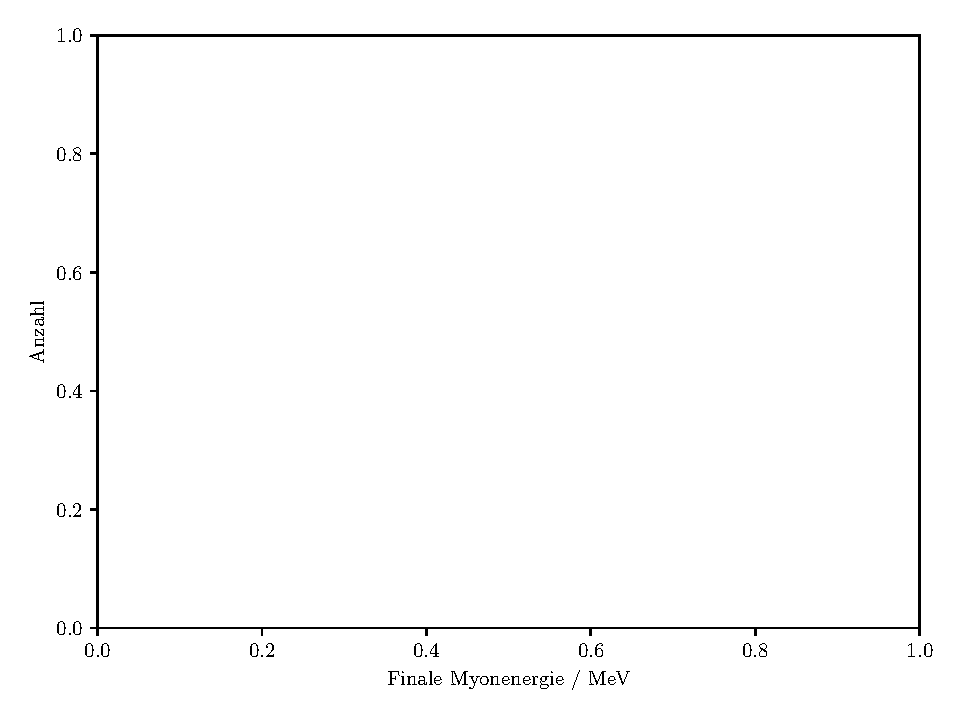
\includegraphics[height=0.9\textheight, trim=0.5cm 0.5cm 0.4cm 0.5cm,clip=true]{plots/cont_rand_0.pdf}}
      \only<2>{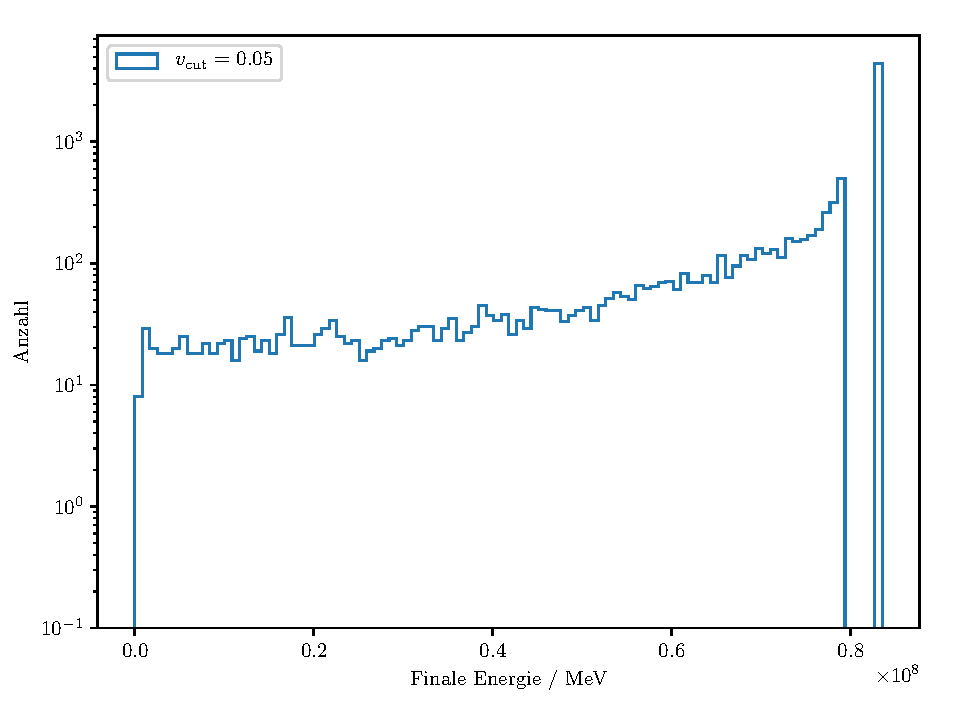
\includegraphics[height=0.9\textheight, trim=0.5cm 0.5cm 0.4cm 0.5cm,clip=true]{plots/cont_rand_1.pdf}}
      \only<3>{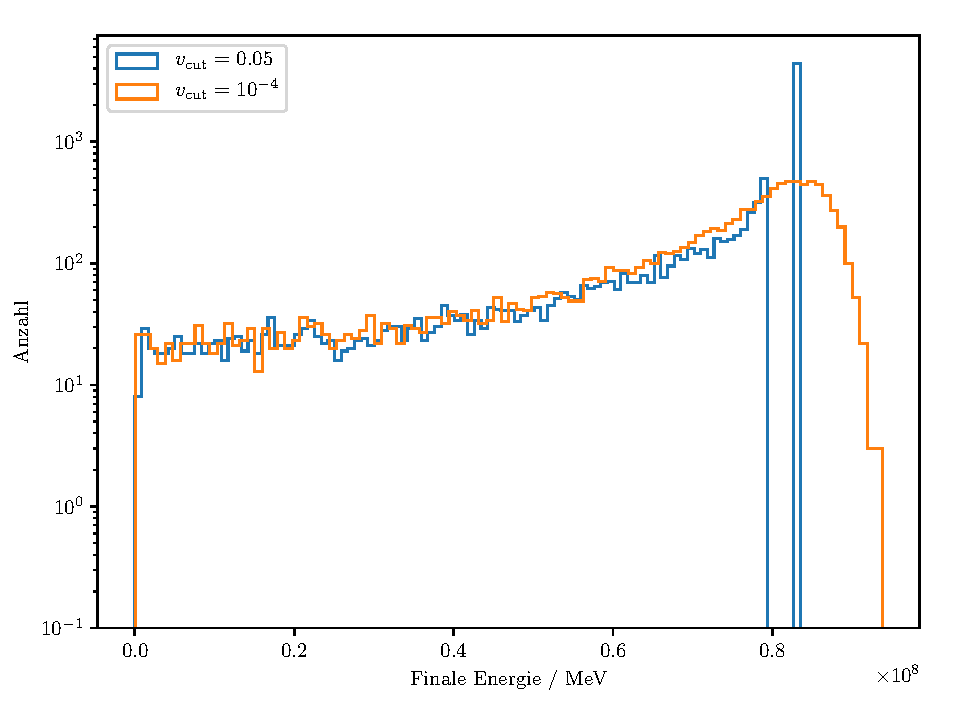
\includegraphics[height=0.9\textheight, trim=0.5cm 0.5cm 0.4cm 0.5cm,clip=true]{plots/cont_rand_2.pdf}}
      \only<4>{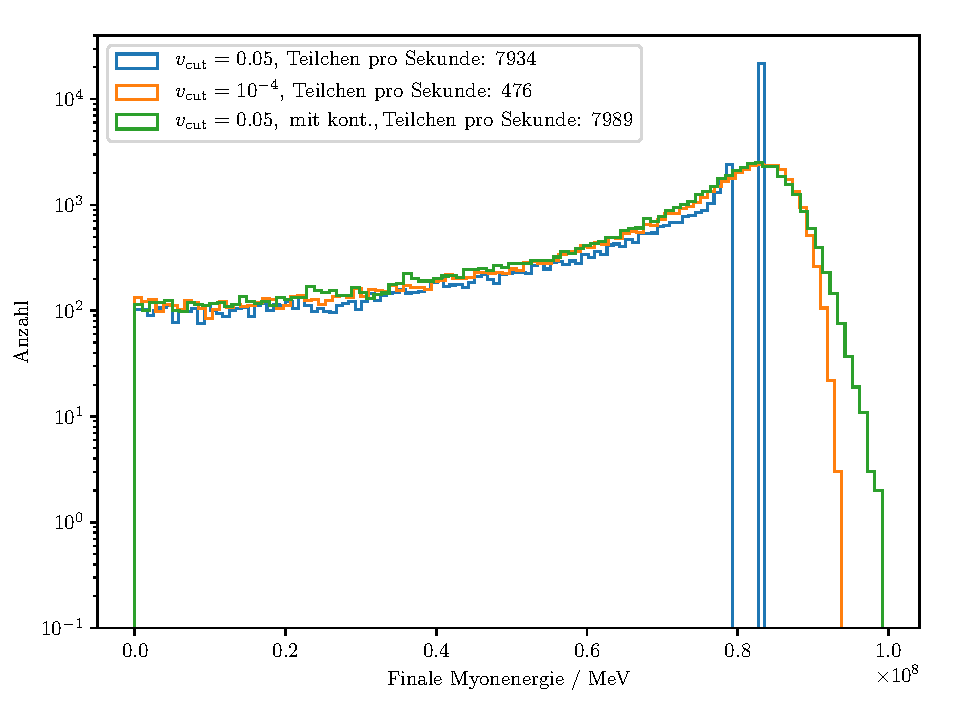
\includegraphics[height=0.9\textheight, trim=0.5cm 0.5cm 0.4cm 0.5cm,clip=true]{plots/cont_rand_3.pdf}}
      \caption*{Propagation von $\num{e4}$ Myonen einer Startenergie von $\SI{e8}{\mega\electronvolt}$ durch $\SI{300}{\metre}$ Stein.}
      \label{fig:1}
      \end{overprint}
  \end{figure}
\end{frame}

\section{Einführung in PROPOSAL - Prozesse}

\begin{frame}
  \begin{figure}
      \centering
      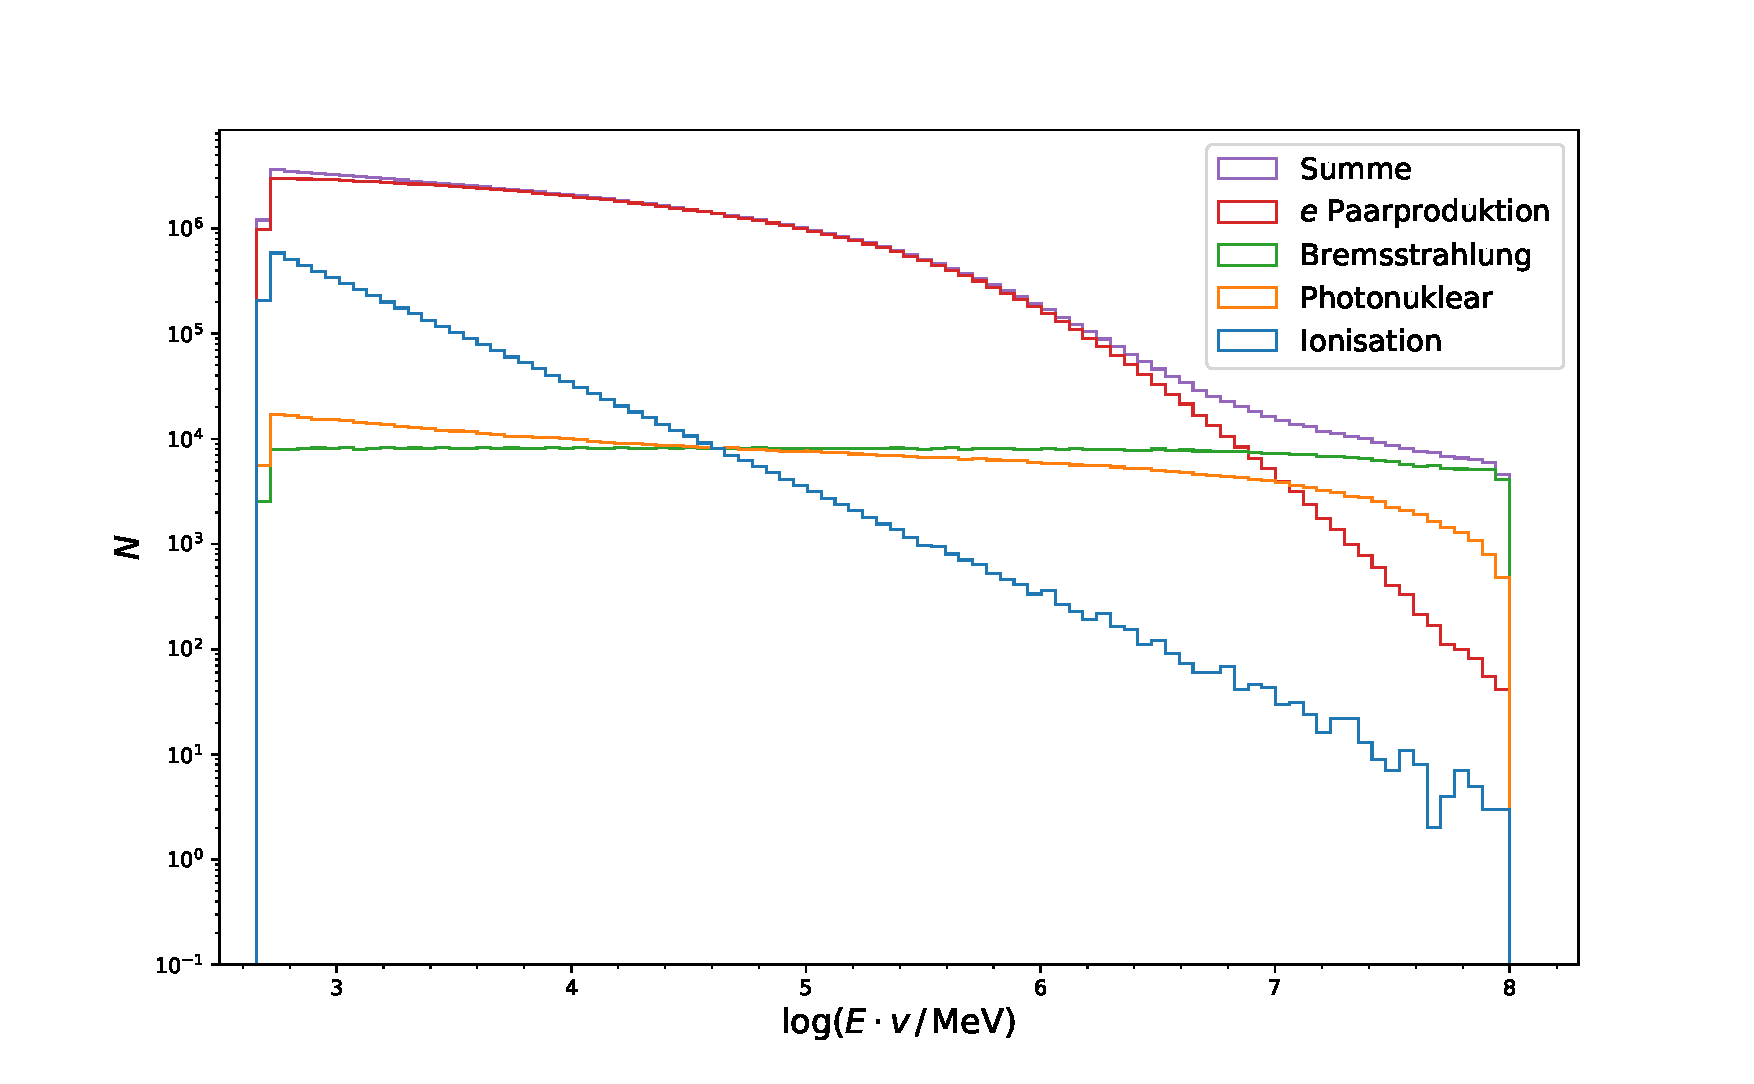
\includegraphics[height=0.9\textheight, trim=0.5cm 0.5cm 0.4cm 2cm,clip=true]{{plots/spectra/all_standardrock_stats_1000000_Emin_8.0_Emax_8.0_index_1}.pdf}
      \caption*{Energieverluste von $\num{e6}$ Myonen einer Startenergie von $\SI{e8}{\mega\electronvolt}$ durch $\SI{100}{\metre}$ Stein.}
      \label{fig:1}
  \end{figure}
\end{frame}

%%% 2. Seltene Prozesse

% Contents slide

\section{}

\begin{frame}[noframenumbering]{Inhalt}
   \begin{columns}
       \begin{column}{0.4\textwidth}

            \setbeamercolor{block title}{fg=white, bg=darkgray}
            \setbeamercolor{block body}{fg=darkgray, bg=gray}

            \begin{block}{1. Einführung in PROPOSAL}
              \centering
                \vspace{2mm}
              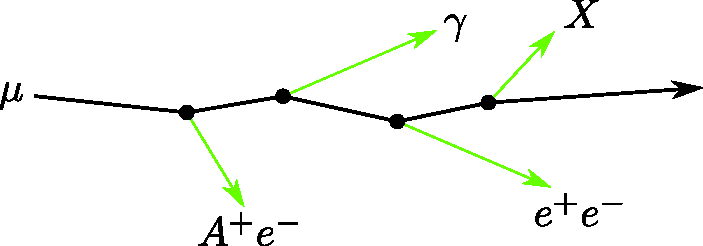
\includegraphics[height=0.15\textheight]{plots/muon_path.pdf}
                \vspace{2mm}
            \end{block}
       \end{column}
       \begin{column}{0.4\textwidth}

            \setbeamercolor{block title}{fg=white, bg=tugreen}
            \setbeamercolor{block body}{fg=darkgray, bg=tulight}

            \begin{block}{2. Seltene Prozesse}
            \centering
            \vspace{2mm}
      \resizebox{!}{0.15\textheight}{%
            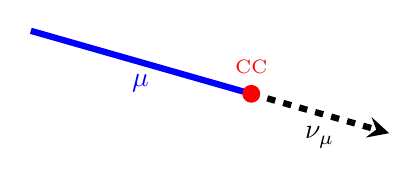
\begin{tikzpicture}
              \centering
                    
            \draw [line width=0.8mm, blue] (-1.9, 1.8) -- node[below] {$\mu$}  (0.9, 1.);     
            \draw [line width=0.8mm, black, dashed, ->, >=stealth] (0.9, 1.) -- node[below] {$\nu_{\mu}$}  (0.9+1.4+0.35, 1. - 0.4 - 0.1);      
            \draw[red,fill=red] (0.9, 1.) circle (0.7ex) node[label=above: $\scriptsize \text{CC}$]{};
          \end{tikzpicture}
        }
      \vspace{3mm}
            \end{block}
       \end{column}
   \end{columns}
   \begin{columns}
       \begin{column}{0.4\textwidth}

            \setbeamercolor{block title}{fg=white, bg=darkgray}
            \setbeamercolor{block body}{fg=darkgray, bg=gray}

            \begin{block}{3. Schauerpropagation}
            \centering
            \vspace{2mm}
      \resizebox{!}{0.15\textheight}{%

            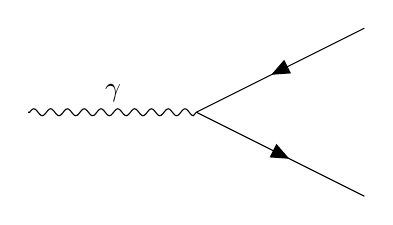
\begin{tikzpicture}
                  \centering
                   % Sizes
                   \pgfmathsetmacro{\len}{0.05cm}
                   \pgfmathsetmacro{\halflen}{\len/4}
                   \pgfmathsetmacro{\vertexsize}{\len/20}
                   \begin{feynman}
                       % vertices
                       \vertex (a) at (0, 0);
                       \vertex (b) at (1.5*\len, 0);
                       \vertex (c) at (3*\len, 0.75*\len);
                       \vertex (d) at (3*\len, -0.75*\len);;
                 
                       % draw diagram
                       \diagram* {
                         (c) -- [fermion] (b) -- [fermion] (d),
                         (a) -- [boson, edge label=\(\gamma\)] (b),
                       };   
                  \end{feynman}
            \end{tikzpicture}
            }
            \vspace{2.5mm}
           \end{block}
       \end{column}
       \begin{column}{0.4\textwidth}

            \setbeamercolor{block title}{fg=white, bg=darkgray}
            \setbeamercolor{block body}{fg=darkgray, bg=gray}

           \begin{block}{4. Ergebnisse}
              \centering
                \vspace{2mm}
              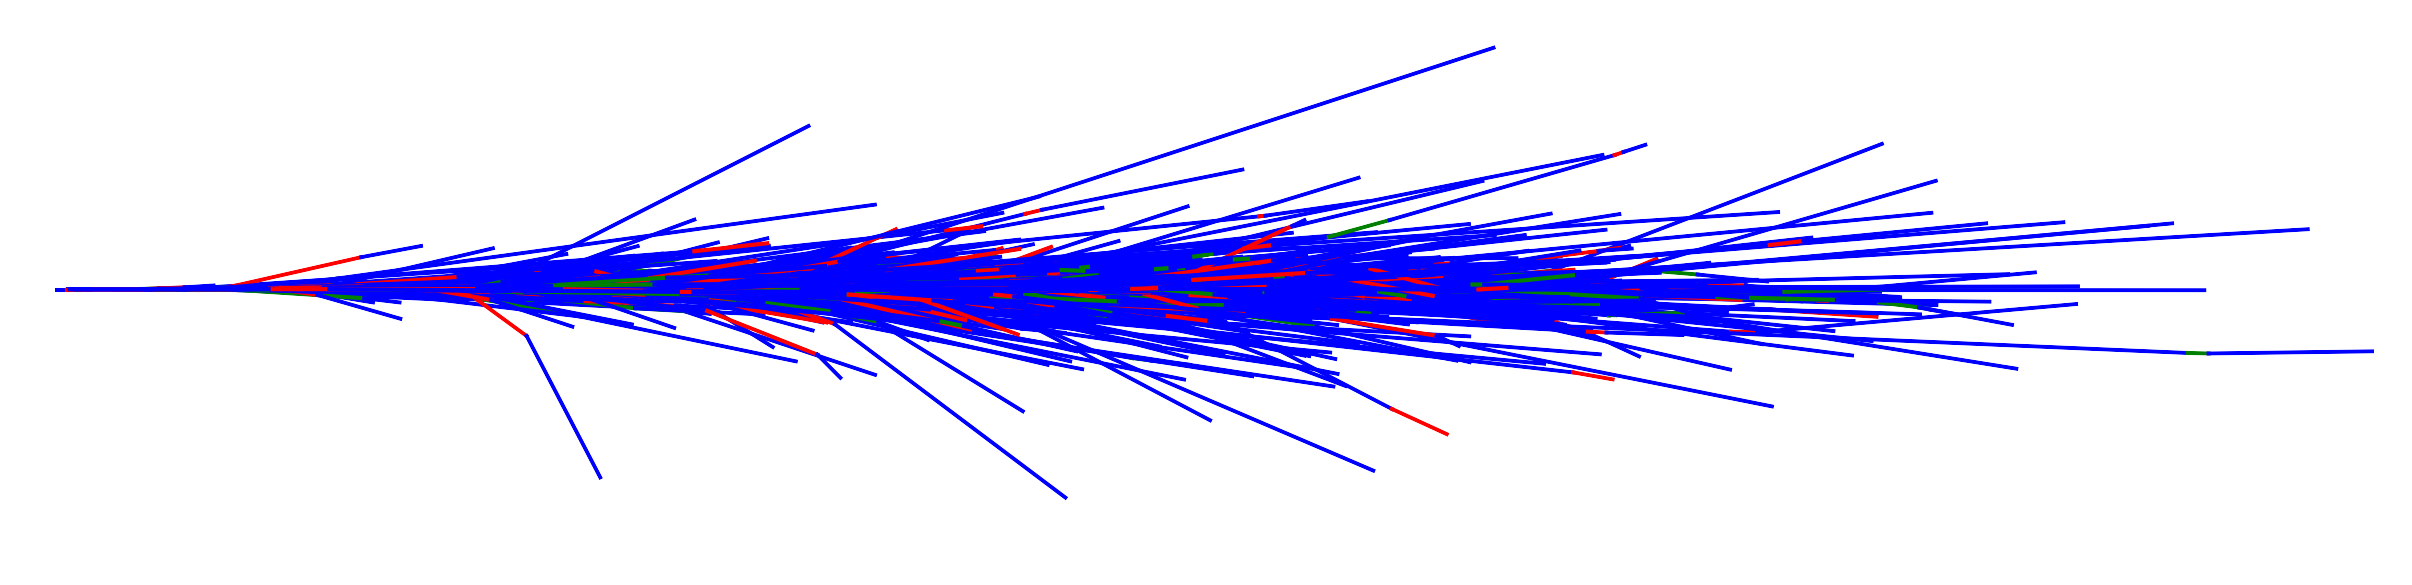
\includegraphics[height=0.15\textheight]{plots/shower_nolegend.png}
                \vspace{2mm}
           \end{block}
       \end{column}
   \end{columns}
\end{frame}

% Myon Paarproduktion

\section{Seltene Prozesse - Myon-Paarproduktion}

\begin{frame}{Myonpaarproduktion}
  \begin{columns}

    \column{0.45\textwidth}
    \begin{center}
      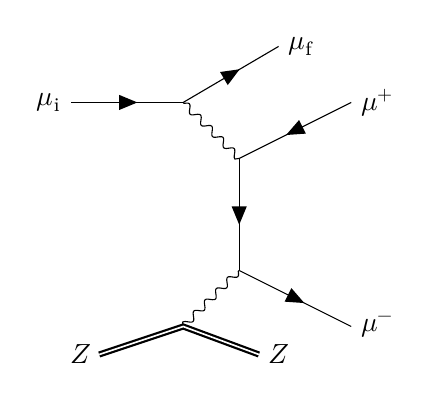
\begin{tikzpicture}
      \centering
       % Sizes
       \pgfmathsetmacro{\len}{0.05cm}
       \pgfmathsetmacro{\halflen}{\len/4}
       \pgfmathsetmacro{\vertexsize}{\len/20}
       \begin{feynman}
           % vertices
           \vertex (a) at (0, 0);
           \vertex (b) at (0, -1*\len);
           \vertex (d) at (-0.5*\len, 0.5*\len);
           \vertex (c) at (-0.5*\len, -1.5*\len);
           \vertex (i1) at (-1.5*\len, 0.5*\len);
           \vertex (i2) at (0, 1.5*\len);
           \vertex (f1) at (\len, 0.5*\len);
           \vertex (f2) at (\len, -1.5*\len);
           \vertex (f3) at (0.5, 1*\len);
           \vertex (z1) at (-1.25*\len, -1.75*\len);
           \vertex (z2) at (0.25, -1.75*\len);
     
           % draw diagram
           \diagram* {
             (i1) -- [fermion] (d) -- [fermion] (f3),
             (d) -- [boson] (a),
             (f1) -- [fermion] (a),
             (a) -- [fermion] (b),
             (b) -- [fermion] (f2),
             (b) -- [boson] (c),
           };
           \draw[thick, double] (z1) -- (c) -- (z2);
     
           % labels
           \node[left] at (i1) {$\mu_\text{i}$};
           \node[right] at (f3) {$\mu_\text{f}$};
           \node[right] at (f1) {$\mu^+$};
           \node[right] at (f2) {$\mu^-$};
           \node[left] at (z1) {$Z$};
           \node[right] at (z2) {$Z$};
      \end{feynman}
    \end{tikzpicture}
  \end{center}
  \column{0.55\textwidth}
    Mit dem auf das Myonpaar übertragenen Energieanteil:
      \begin{align*}
        v = \frac{\left( \epsilon_+ + \epsilon_- \right)}{E} \\[-0.3cm]
      \end{align*}

    Mit dem Asymmetrieparameter:
    \begin{align*}
      \rho = \frac{\left( \epsilon_+ - \epsilon_- \right)}{\left( \epsilon_+ + \epsilon_- \right)} \\[-0.3cm]
    \end{align*}

    $E$: Initialenergie des eingehenden Myons $\mu_\text{i}$ \\
    $\epsilon_\pm$: Energie des erzeugten (Anti)myon\\
    $Z$: Atom(kern) im Medium

  \end{columns}
\end{frame}


\begin{frame}{Differentieller Wirkungsquerschnitt}

Analytische, approximative Formel für die Myonpaarproduktion\footnote{Kelner, Kokoulin, Petrukhin: Phys. of Atomic Nuclei, Vol. 63, No. 9, 2000, pp. 1603-1611}:
\begin{align*}
  \frac{\mathrm{d}\sigma}{\mathrm{d}v \mathrm{d}\rho} &= \frac{2}{3\pi} (Z \alpha r_\mu)^2 \frac{1-v}{v} \Phi(v, \rho) \ln \left( X \left(E, v, \rho \right) \right)
\end{align*}

\vspace{5mm}

Abweichungen $\epsilon$ zur exakten Formel:
\begin{itemize}
	\item $\epsilon < 2\textendash3\si{\percent}$ für $E > \SI{30}{\giga\electronvolt}$
	\item $\epsilon < 10\si{\percent}$ für $E < \SI{10}{\giga\electronvolt}$
\end{itemize}
  
\end{frame}


\begin{frame}
  \begin{figure}
      \centering
      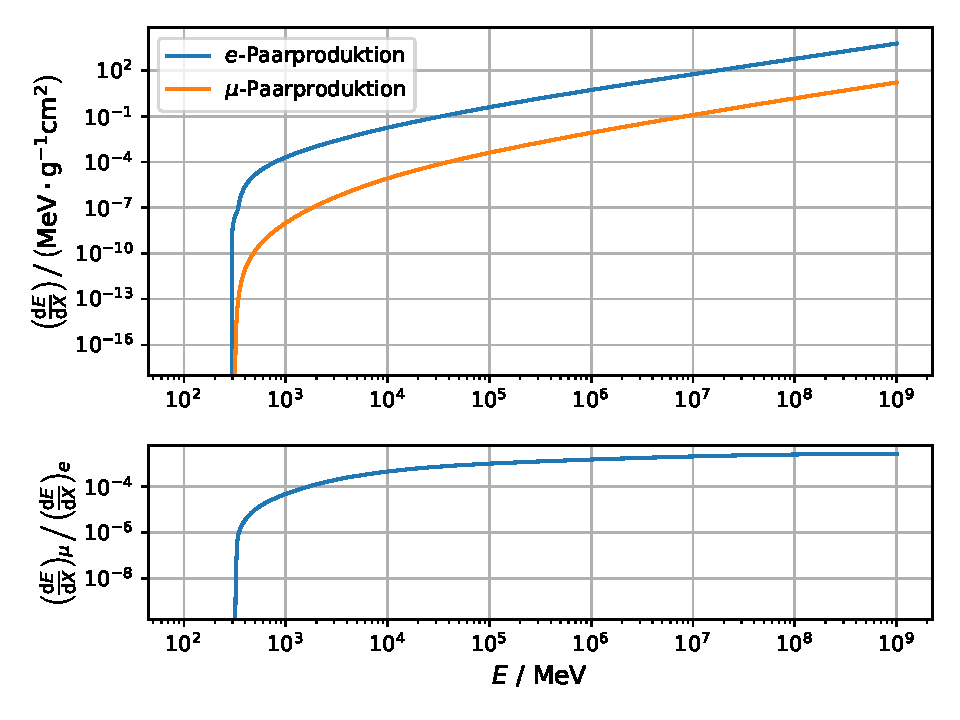
\includegraphics[height=0.9\textheight, trim=0.5cm 0.5cm 0.4cm 0.2cm,clip=true]{{plots/mupair_compare/mupair_compare}.pdf}
      \caption*{Vergleich der kontinuierlichen Energieverluste (d.h. $v_\text{cut} = v_\text{max}$) in Stein.}
      \label{fig:1}
  \end{figure}
\end{frame}


\begin{frame}
  \begin{figure}
      \centering
      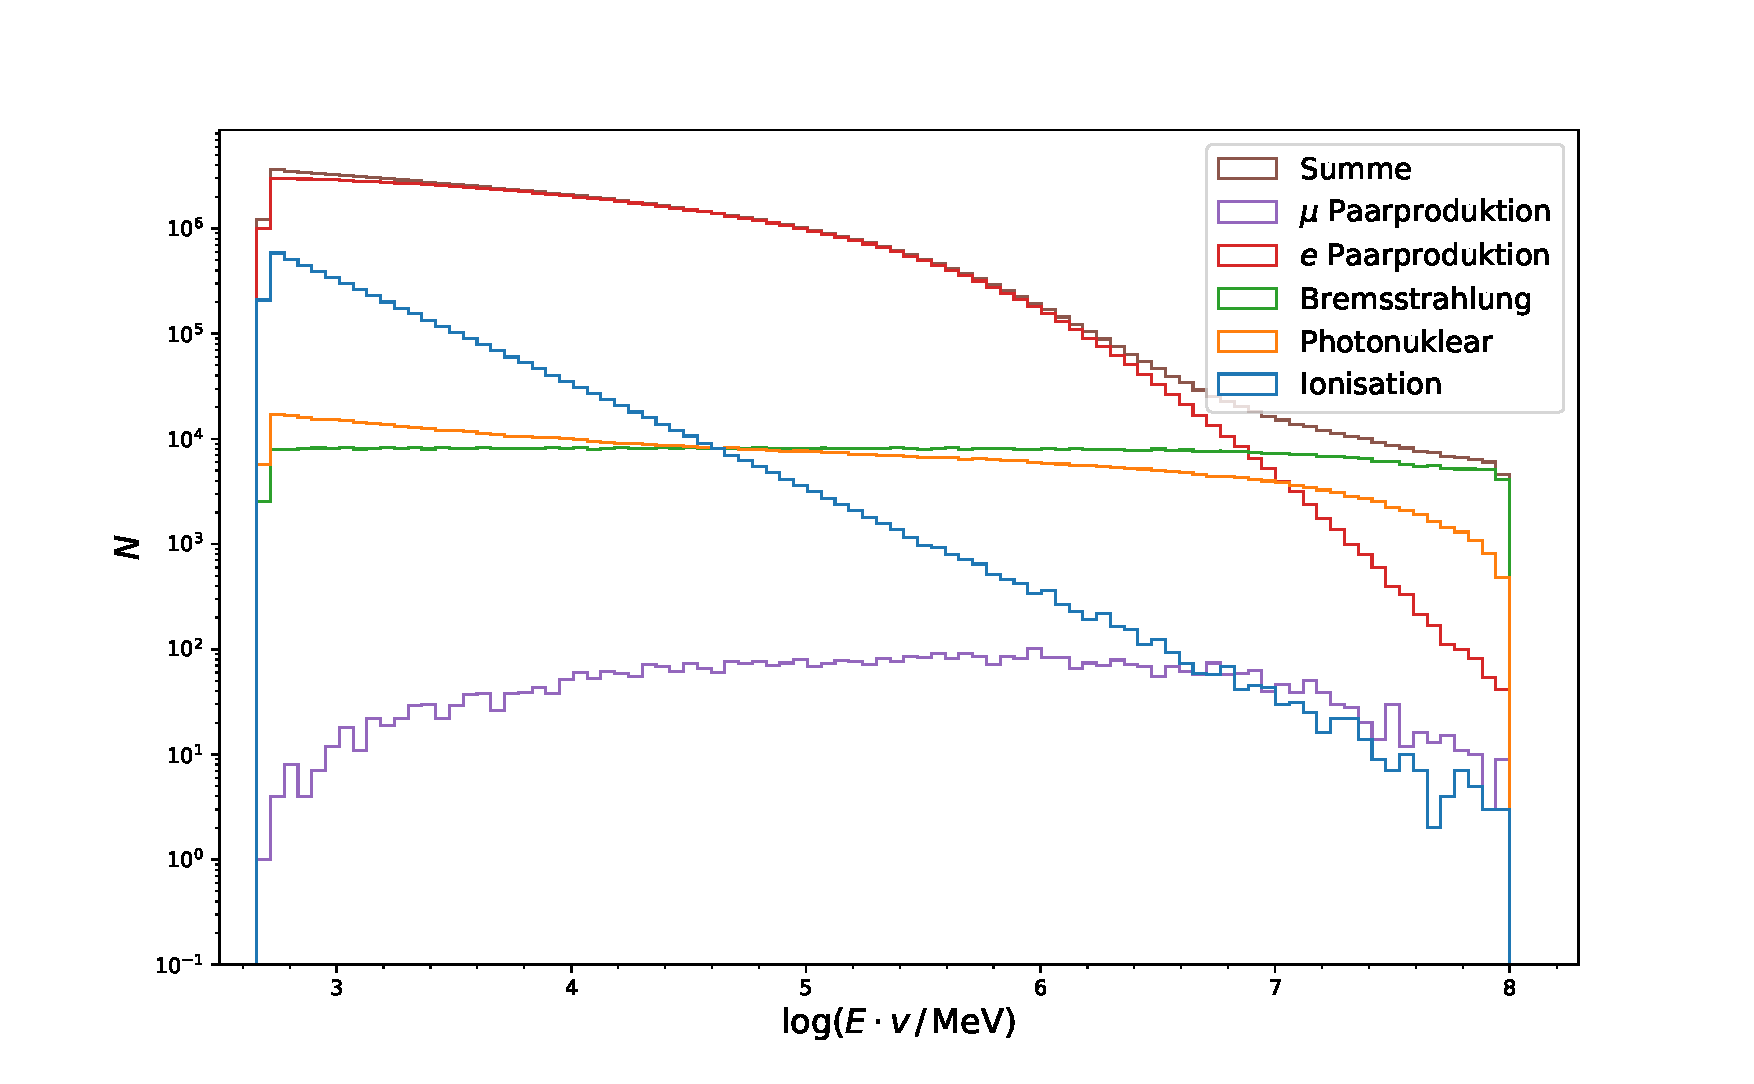
\includegraphics[height=0.9\textheight, trim=0.5cm 0.5cm 0.4cm 2cm,clip=true]{{plots/spectra/all_mupair_standardrock_stats_1000000_Emin_8.0_Emax_8.0_index_1}.pdf}
      \caption*{Energieverluste von $\num{e6}$ Myonen einer Startenergie von $\SI{e8}{\mega\electronvolt}$ durch $\SI{100}{\metre}$ Stein.}
      \label{fig:1}
  \end{figure}
\end{frame}


\begin{frame}{Relevanz}
	\textbf{IceCube-Ereignisse}
	 \begin{itemize}
	 	\setlength\itemsep{0.5em}
	 	\item "Energieverluste" aufgrund von Myonpaarproduktion vernachlässigbar
	 	\item Veränderte Signatur von einem Myon-Bündel im Vergleich zu einem einzelnen hochenergetischen Myon 
	 \end{itemize}
\end{frame}


\begin{frame}{Relevanz}
	 \textbf{Luftschauer}\footnote{Kudryavtsev, Korolkova, Spooner: Physical Letter B 471, 1999, pp. 251-256}
	 \begin{itemize}
	 	\setlength\itemsep{0.5em}	 	
	 	\item Zwei mögliche Quellen für Myon-Bündel in Untergrundexperimenten:
	 	\begin{itemize}
	 		\item[$\rightarrow$] Hardronische Komponente in Luftschauern
	 		\item[$\rightarrow$] Myonpaarproduktion in Stein/Wasser
	 	\end{itemize}
	 	\vspace{5mm}
	 	\item Messe Anzahl und Eigenschaften von Myon-Bündeln
	 	\begin{itemize}
	 		\item[$\rightarrow$] Informationen über hadronische Wechselwirkungsmodelle
	 		\item[$\rightarrow$] Informationen über Schauerkomposition
	 	\end{itemize}
	 \end{itemize}
\end{frame}

% Schwache Wechselwirkung

\section{Seltene Prozesse - Schwache Wechselwirkung}

\begin{frame}{Schwache Wechselwirkung}
  \begin{columns}

    \column{0.45\textwidth}
    \begin{center}
      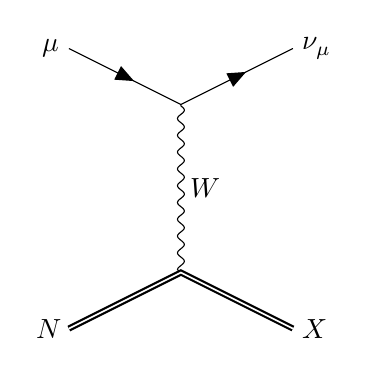
\begin{tikzpicture}
      \centering
       % Sizes
       \pgfmathsetmacro{\len}{0.05cm}
       \pgfmathsetmacro{\halflen}{\len/4}
       \pgfmathsetmacro{\vertexsize}{\len/20}
       \begin{feynman}
           % vertices
           \vertex (a) at (-1*\len, 0.5*\len);
           \vertex (b) at (0, 0);
           \vertex (c) at (1*\len, 0.5*\len);
           \vertex (d) at (0, -1.5*\len);
           \vertex (e) at (-1*\len, -2*\len);
           \vertex (f) at (1*\len, -2*\len);
     
           % draw diagram
           \diagram* {
             (a) -- [fermion] (b) -- [fermion] (c),
             (b) -- [boson, edge label=\(W\)] (d),

           };
           \draw[thick, double] (e) -- (d) -- (f);
     
           % labels
           \node[left] at (a) {$\mu$};
           \node[right] at (c) {$\nu_{\mu}$};
           %\node[right] at (f1) {$\mu^+$};
           %\node[right] at (f2) {$\mu^-$};
           \node[left] at (e) {$N$};
           \node[right] at (f) {$X$};
      \end{feynman}
    \end{tikzpicture}
  \end{center}

  \column{0.56\textwidth}
    \begin{itemize}
      \item Stark unterdrückter Prozess
      \item Rein stochastische Wechselwirkung (d.h. $v_\text{cut} = v_\text{min}$, kein Beitrag zu kontinuierlichen Verlusten)
      \item Erhalte Wirkungsquerschnitt aus Crossing-Symmetrie:
      \begin{align*}
        \mathrm{d}\sigma\left( \mu N \rightarrow \nu_\mu X \right) = \frac{1}{2} \mathrm{d}\sigma\left( \nu_\mu X \rightarrow \mu N \right)
      \end{align*}
    \end{itemize}
  \end{columns}
\end{frame}


\begin{frame}
  \begin{columns}

    \column{0.45\textwidth}
    \begin{center}
    \begin{figure}
      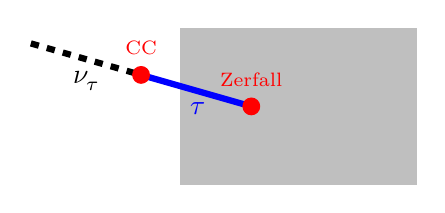
\begin{tikzpicture}
      \centering
       
      \fill [lightgray] (0.0, 0.0) rectangle (3.0, 2.0);

	  \draw [line width=0.8mm, blue] (-0.5, 1.4) -- node[below] {$\tau$}  (0.9, 1.);

	  \draw [line width=0.8mm, black, dashed] (-1.9, 1.8) -- node[below] {$\nu_{\tau}$}  (-0.5, 1.4);

	  \draw[red,fill=red] (0.9, 1.) circle (0.7ex) node[label=above: $\scriptsize \text{Zerfall}$]{};

	  \draw[red,fill=red] (-0.5, 1.4) circle (0.7ex) node[label=above: $\scriptsize \text{CC}$]{};

	  %\draw [->,>=stealth, line width=0.4mm, red] (1.25-0.175, 0.9+0.05) --  (1.25+0.175, 0.9-0.05);
	  %\draw [->,>=stealth, line width=0.4mm, red] (1.25-0.175, 0.9+0.05) --  (1.25+0.175, 0.9-0.15);
	  %\draw [line width=0.4mm, red] (1.25-0.175, 0.9+0.05) ->  (1.25+0.175, 0.9);
    \end{tikzpicture}
    \caption*{Lollipop-Signatur von $\tau$-Neutrinos}
  \end{figure}
  \end{center}

  \begin{center}
    \begin{figure}
      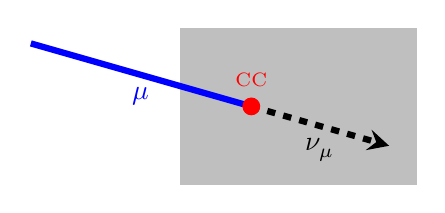
\begin{tikzpicture}
      \centering
       
      \fill [lightgray] (0.0, 0.0) rectangle (3.0, 2.0);

	  \draw [line width=0.8mm, blue] (-1.9, 1.8) -- node[below] {$\mu$}  (0.9, 1.);

	  \draw [line width=0.8mm, black, dashed, ->, >=stealth] (0.9, 1.) -- node[below] {$\nu_{\mu}$}  (0.9+1.4+0.35, 1. - 0.4 - 0.1);

	  \draw[red,fill=red] (0.9, 1.) circle (0.7ex) node[label=above: $\scriptsize \text{CC}$]{};

	  %\draw [->,>=stealth, line width=0.4mm, red] (1.25-0.175, 0.9+0.05) --  (1.25+0.175, 0.9-0.05);
	  %\draw [->,>=stealth, line width=0.4mm, red] (1.25-0.175, 0.9+0.05) --  (1.25+0.175, 0.9-0.15);
	  %\draw [line width=0.4mm, red] (1.25-0.175, 0.9+0.05) ->  (1.25+0.175, 0.9);
    \end{tikzpicture}
    \caption*{Schwache Wechselwirkung von Myonen}
  \end{figure}
  \end{center}

  \column{0.56\textwidth}
    \begin{itemize}
      \item Ähnlichkeiten mit hochenergetischen $\tau$-Events ("Lollipop-Signatur")
      \item Möglicher Untergrund von bis zu $\SI{10}{\percent}$ bei Suchen nach $\tau$-Lollipop-Events in IceCube\footnotemark
    \end{itemize}
  \end{columns}
  \footnotetext{Sandrock, Alexander: Higher-order corrections to the energy loss cross sections of high-energy muons, 2018, pp. 38-40}
\end{frame}

%%% 3. Schauerpropagation

% Contents slide

\section{}

\begin{frame}[noframenumbering]{Inhalt}
   \begin{columns}
       \begin{column}{0.4\textwidth}

            \setbeamercolor{block title}{fg=white, bg=darkgray}
            \setbeamercolor{block body}{fg=darkgray, bg=gray}

            \begin{block}{1. Einführung in PROPOSAL}
              \centering
                \vspace{2mm}
              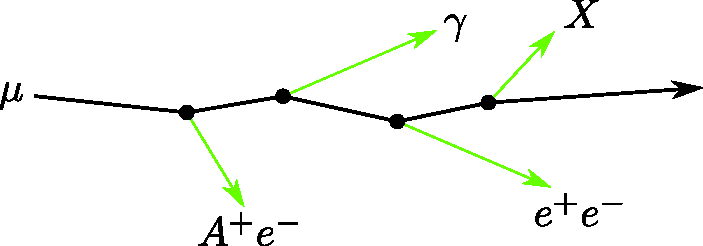
\includegraphics[height=0.15\textheight]{plots/muon_path.pdf}
                \vspace{2mm}
            \end{block}
       \end{column}
       \begin{column}{0.4\textwidth}

            \setbeamercolor{block title}{fg=white, bg=darkgray}
            \setbeamercolor{block body}{fg=darkgray, bg=gray}

            \begin{block}{2. Seltene Prozesse}
            \centering
            \vspace{2mm}
      \resizebox{!}{0.15\textheight}{%
            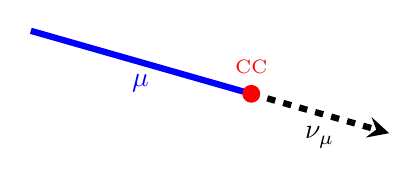
\begin{tikzpicture}
              \centering
                    
            \draw [line width=0.8mm, blue] (-1.9, 1.8) -- node[below] {$\mu$}  (0.9, 1.);     
            \draw [line width=0.8mm, black, dashed, ->, >=stealth] (0.9, 1.) -- node[below] {$\nu_{\mu}$}  (0.9+1.4+0.35, 1. - 0.4 - 0.1);      
            \draw[red,fill=red] (0.9, 1.) circle (0.7ex) node[label=above: $\scriptsize \text{CC}$]{};
          \end{tikzpicture}
        }
      \vspace{3mm}
            \end{block}
       \end{column}
   \end{columns}
   \begin{columns}
       \begin{column}{0.4\textwidth}

            \setbeamercolor{block title}{fg=white, bg=tugreen}
            \setbeamercolor{block body}{fg=darkgray, bg=tulight}

            \begin{block}{3. Schauerpropagation}
            \centering
            \vspace{2mm}
      \resizebox{!}{0.15\textheight}{%

            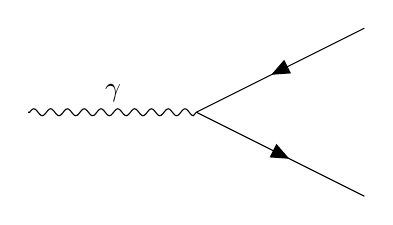
\begin{tikzpicture}
                  \centering
                   % Sizes
                   \pgfmathsetmacro{\len}{0.05cm}
                   \pgfmathsetmacro{\halflen}{\len/4}
                   \pgfmathsetmacro{\vertexsize}{\len/20}
                   \begin{feynman}
                       % vertices
                       \vertex (a) at (0, 0);
                       \vertex (b) at (1.5*\len, 0);
                       \vertex (c) at (3*\len, 0.75*\len);
                       \vertex (d) at (3*\len, -0.75*\len);;
                 
                       % draw diagram
                       \diagram* {
                         (c) -- [fermion] (b) -- [fermion] (d),
                         (a) -- [boson, edge label=\(\gamma\)] (b),
                       };   
                  \end{feynman}
            \end{tikzpicture}
            }
            \vspace{2.5mm}
           \end{block}
       \end{column}
       \begin{column}{0.4\textwidth}

            \setbeamercolor{block title}{fg=white, bg=darkgray}
            \setbeamercolor{block body}{fg=darkgray, bg=gray}

           \begin{block}{4. Ergebnisse}
              \centering
                \vspace{2mm}
              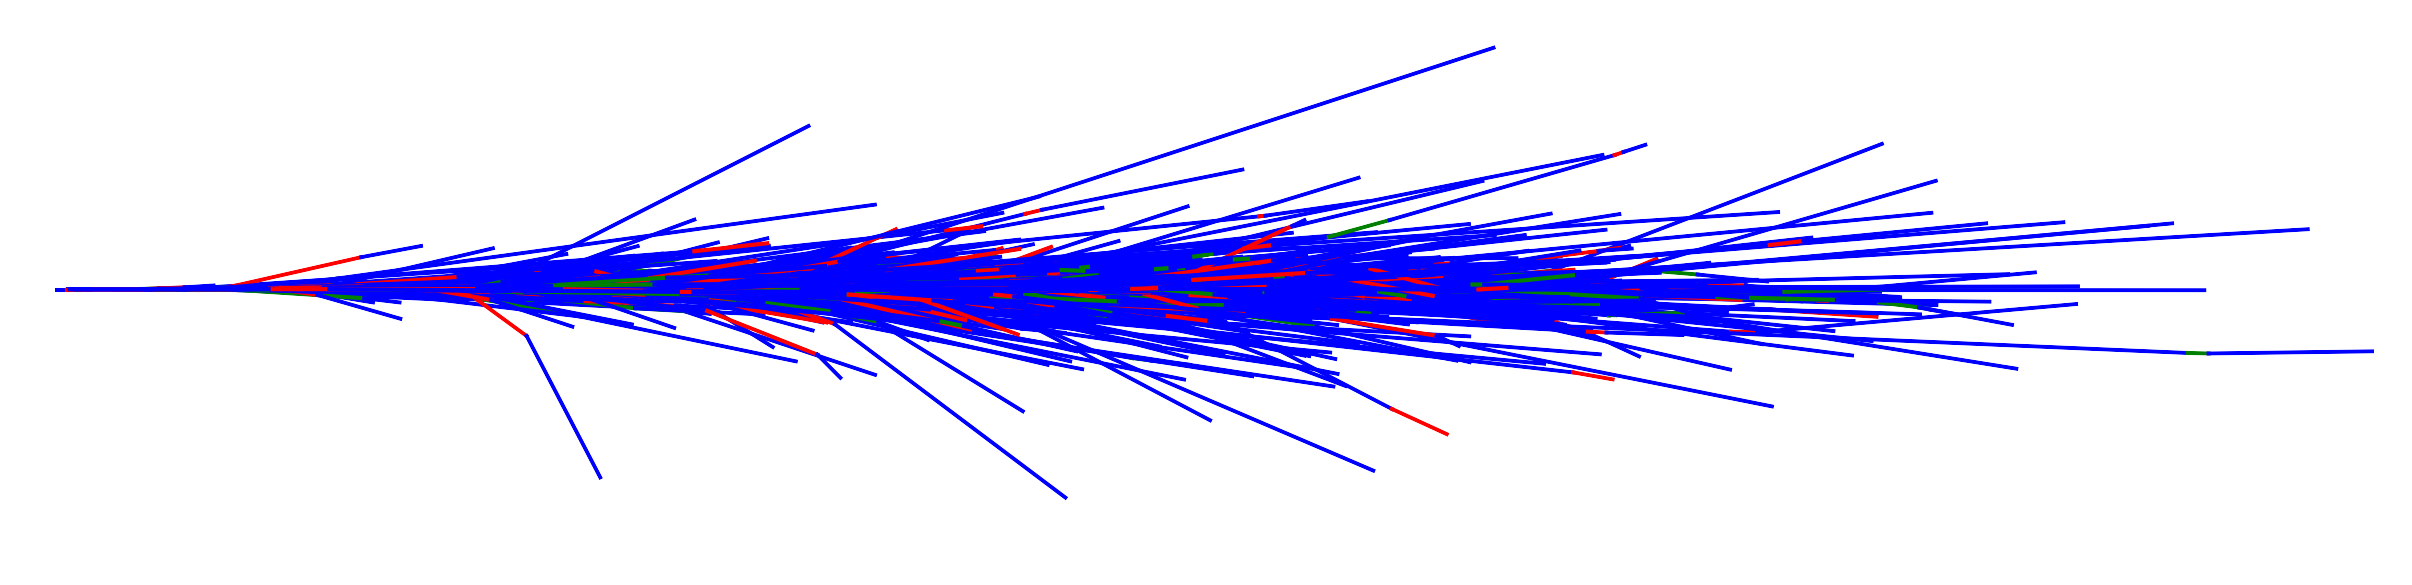
\includegraphics[height=0.15\textheight]{plots/shower_nolegend.png}
                \vspace{2mm}
           \end{block}
       \end{column}
   \end{columns}
\end{frame}

\section{Schauerpropagation - Einführung}


\begin{frame}
  \begin{figure}
      \centering
      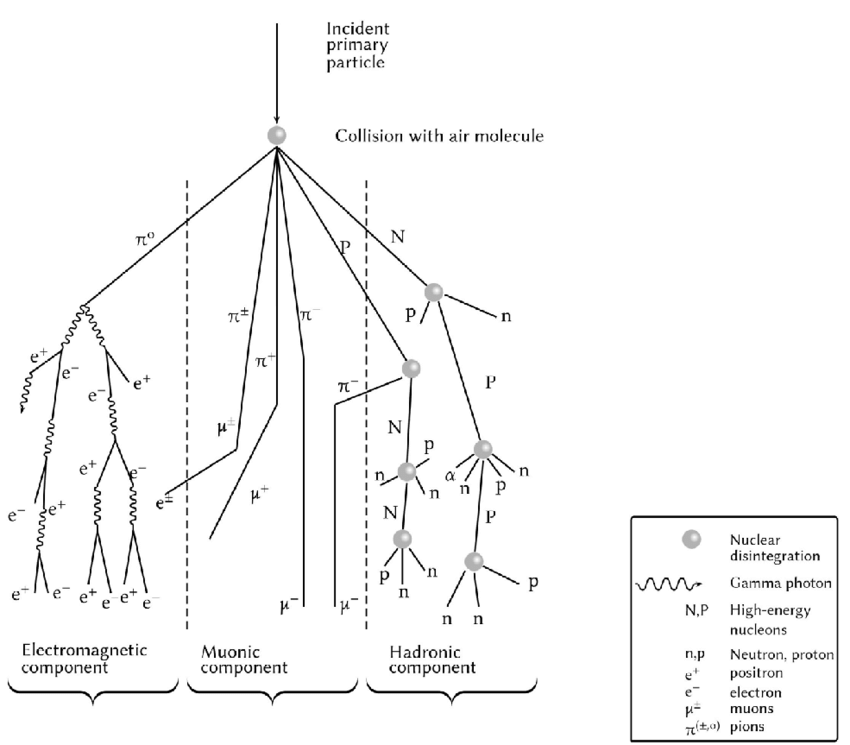
\includegraphics[height=0.80\textheight, trim=0.0cm 2.4cm 8.0cm 0.5cm,clip=true]{{plots/shower}.png}
      \caption*{Skizze der Komponenten eines Luftschauers\footnotemark.}
      \label{fig:1}
  \end{figure}
  \footnotetext{Geofísica Internacional 57(4):253-275, October 2018}
\end{frame}


\begin{frame}
  \begin{columns}
    \column{0.6\textwidth}
    \begin{center}
      \begin{itemize}
        \setlength\itemsep{0.5em}
        \item \textbf{CORSIKA}: Programm zur Simulation von Teilchenschauern
        \item Verschiedene Modelle zur Beschreibung der hadronischen Wechselwirkungen
        \item Beschreibung der elektromagnetischen Wechselwirkungen durch \textbf{EGS4}
        \begin{itemize}
          \item[$\rightarrow$] Ziel: Ermögliche Nutzung von \textbf{PROPOSAL} in \textbf{CORSIKA 8}
          \item[$\rightarrow$] Aufgabe: Propagation von $e^+$, $e^-$ und $\gamma$ in \textbf{PROPOSAL}
        \end{itemize}
      \end{itemize}
  \end{center}
  \column{0.4\textwidth}
      \begin{figure}
          \centering
          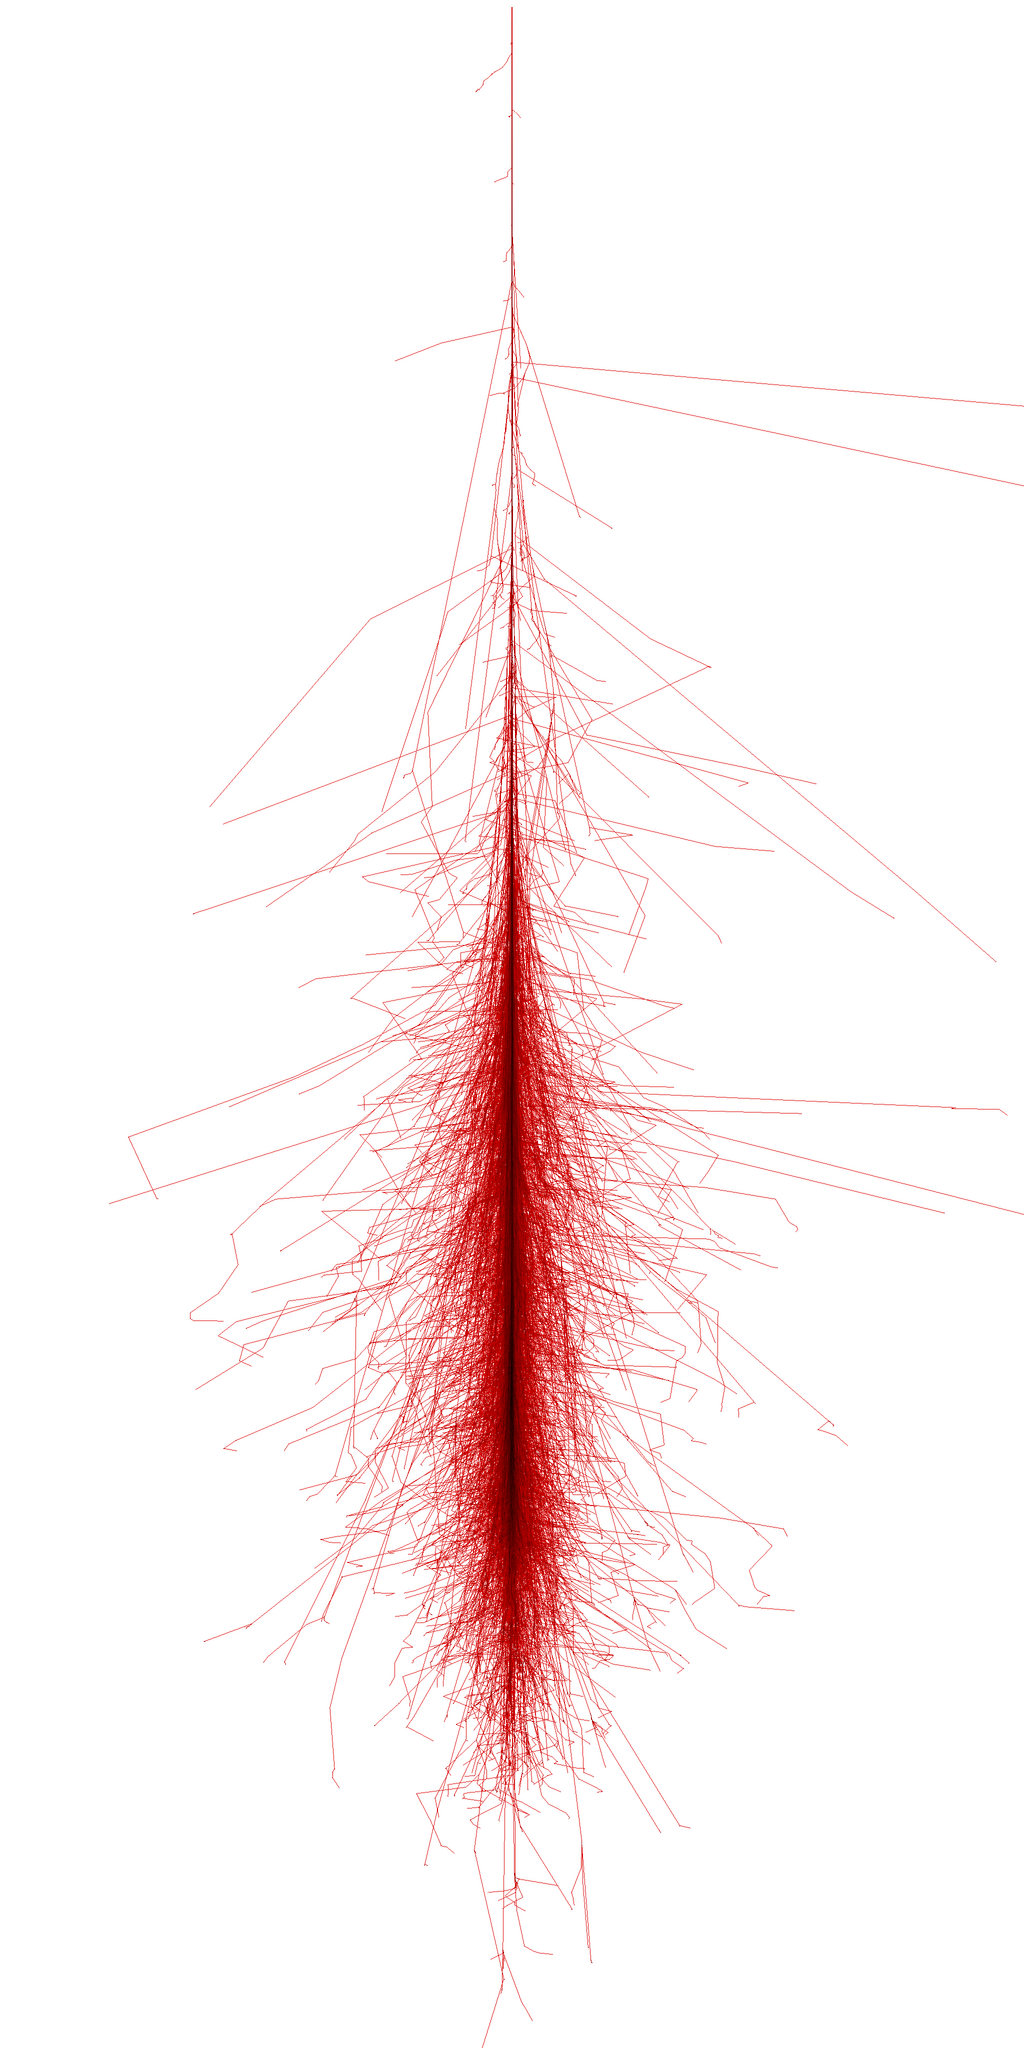
\includegraphics[width=0.4\linewidth]{plots/corsika.png}
           \captionsetup{format=myformat}
          \caption*{Projektion eines Luftschauers, initiiert durch ein $\SI{100}{\giga\electronvolt}$ Photon\footnotemark.}
      \end{figure}
  \end{columns}
\footnotetext{F. Schmidt, J. Knapp, https://www-zeuthen.desy.de/~jknapp/fs/showerimages.html}
\end{frame}


\section{Schauerpropagation - $e^-$ und $e^+$ Propagation}

% Ionisation

\begin{frame}{Ionisation}
	 \begin{itemize}
	 	\setlength\itemsep{0.5em}
	 	\item Energieverlust durch inelastische Stöße mit Hüllenelektronen
	 	\item \textbf{Bethe-Formel}: Beschreibt Ionisationsverluste schwerer geladener Teilchen
	 	\begin{itemize}
          \item[$\rightarrow$] Modifizierte Formel für $\mu$ und $\tau$ in PROPOSAL
	 	\end{itemize}
	 	\vspace{5mm}
	 	\item Bethe-Formel nicht direkt für $e^-$/$e^+$ anwendbar:
	 	\begin{itemize}
          \item[$\rightarrow$] Ununterscheidbarkeit der beteiligten Teilchen
          \item[$\rightarrow$] Identische Massen der beteiligten Teilchen
	 	\end{itemize}
	 \end{itemize}
\end{frame}


\begin{frame}
	 \begin{itemize}
	 	\setlength\itemsep{0.5em}
	 	\item Für ausreichend \emph{hohe Energieüberträge} können atomare Elektronen als frei betrachtet werden
	 	\begin{itemize}
          \item[$\rightarrow$] Ionisation als Bhabha-Streuung ($ e^+ + e^- \rightarrow e^+ + e^- $)
          \item[$\rightarrow$] Ionisation als Møller-Streuung ($ e^- + e^- \rightarrow e^- + e^- $)
	 	\end{itemize}
        \item Für \emph{kleine Energieüberträge} muss explizit über die atomaren Anregungswahrscheinlichkeiten summiert werden
		\item[$\Rightarrow$]Erhalte \textbf{Berger-Seltzer Formel}
	 \end{itemize}
\end{frame}


\begin{frame}
  \begin{figure}
      \centering
      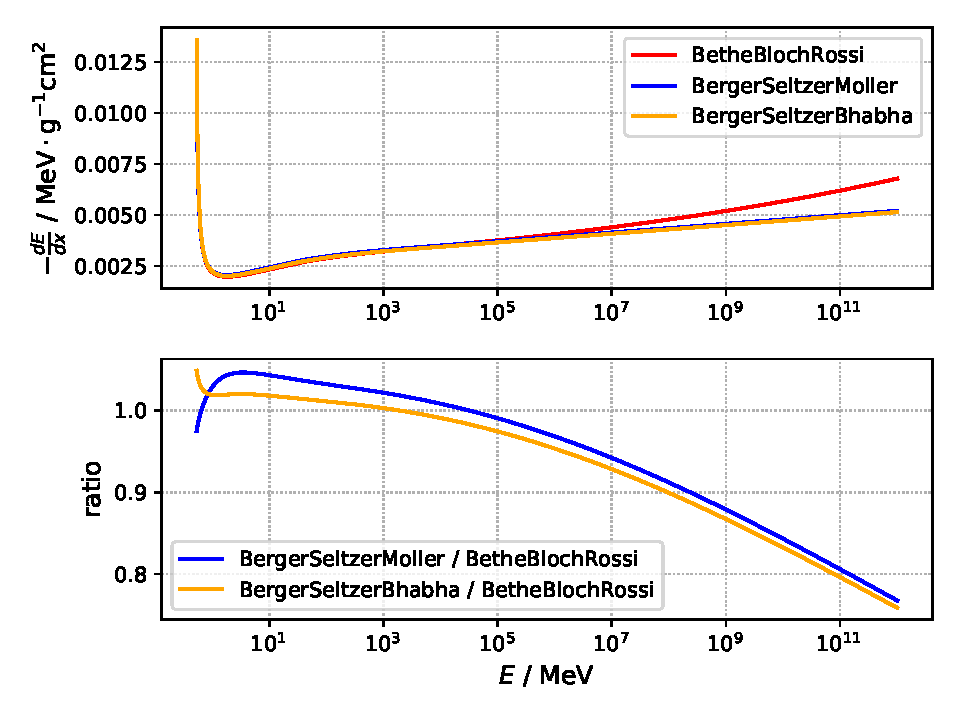
\includegraphics[height=0.9\textheight, trim=0.5cm 0.5cm 0.4cm 0.2cm,clip=true]{{plots/dEdx_all}.pdf}
      \caption*{Vergleiche Ionisationsverluste für $e^-$ und $e^+$ mit verschiedenen Parametrisierungen.}
      \label{fig:1}
  \end{figure}
\end{frame}

% Bremsstrahlung


\begin{frame}{Bremsstrahlung}
	 \begin{itemize}
	 	\setlength\itemsep{0.5em}
    \item Bremsstrahlung dominierende Wechselwirkung für Elektronen und Positronen
	 	\item \textbf{PROPOSAL} empfiehlt \emph{Complete Screening} als Wirkungsquerschnitt für hochenergetische Elektronen
	 	\item \textbf{EGS4} benutzt energieabhängige Wirkungsquerschnitte:
	 	\begin{itemize}
	 		\item[$\rightarrow$] $E>\SI{50}{\mega\electronvolt}$: Vergleichbar mit \emph{Complete Screening}
	 		\item[$\rightarrow$] $E<\SI{50}{\mega\electronvolt}$: Empirische Korrekturfaktoren für niedrige Energien
	 	\end{itemize}
	 	\item[$\Rightarrow$] Vergleiche verschiedene Implementationen
	 \end{itemize}
\end{frame}



\begin{frame}
  \begin{figure}
      \centering
      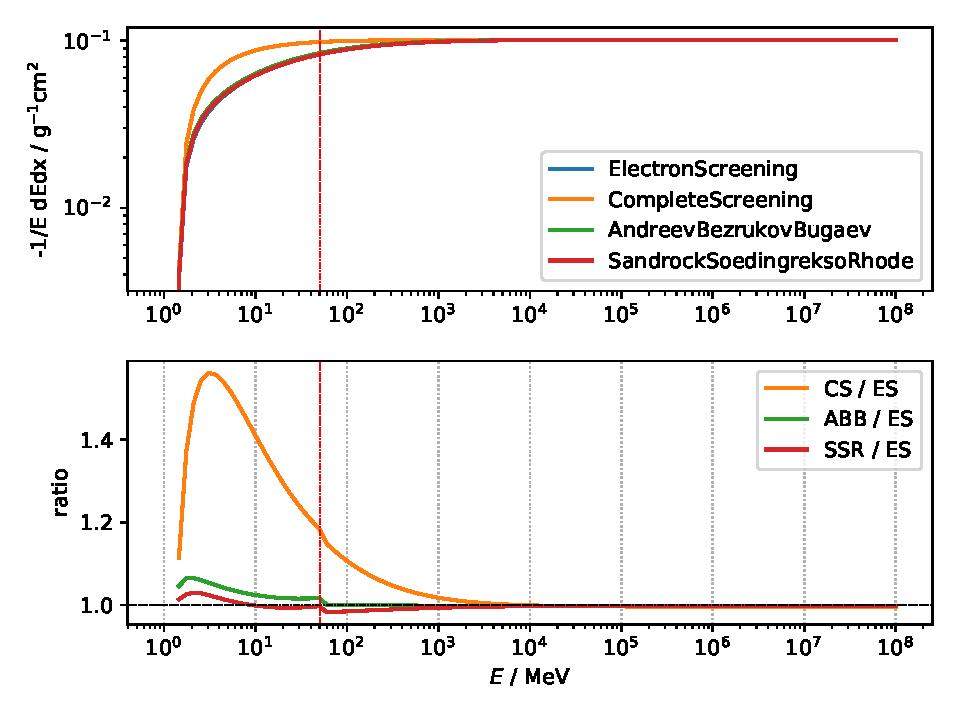
\includegraphics[height=0.9\textheight, trim=0.3cm 0.5cm 0.4cm 0.2cm,clip=true]{{plots/brems/brems_dEdx_sr}.pdf}
      \caption*{Vergleiche Bremsstrahlungsverluste für Elektronen für verschiedene Parametrisierungen.}
      \label{fig:1}
  \end{figure}
\end{frame}

% Annihilation


\begin{frame}{Annihilation}
  \begin{columns}

    \column{0.45\textwidth}
    \begin{center}
      \begin{tikzpicture}
      \centering
       % Sizes
       \pgfmathsetmacro{\len}{0.05cm}
       \pgfmathsetmacro{\halflen}{\len/4}
       \pgfmathsetmacro{\vertexsize}{\len/20}
       \begin{feynman}
           % vertices
           \vertex (c) at (0, 0);
           \vertex (b) at (0, -1.5*\len);
           \vertex (a) at (-1*\len, -2*\len);
           \vertex (f) at (+1*\len, -2*\len);
           \vertex (d) at (-1*\len, 0.5*\len);
           \vertex (e) at (+1*\len, 0.5*\len);
     
           % draw diagram
           \diagram* {
             (a) -- [fermion] (b) -- [fermion] (c) -- [fermion] (d),
             (c) -- [boson, edge label=\(\gamma\)] (e),
             (b) -- [boson, edge label=\(\gamma\)] (f)
           };

           % labels
           \node[left] at (d) {$e^+$};
           \node[left] at (a) {$e^-$};
      \end{feynman}
    \end{tikzpicture}
  \end{center}

  \column{0.56\textwidth}
    \begin{itemize}
      \item Annihilation eines Positrons mit einem atomaren Elektron
      \item Annahme: Atomares Elektron frei und in Ruhe
      \item Rein stochastische Wechselwirkung
      \item (Polar)-Winkel vollständig kinematisch bestimmt (2 \rightarrow 2 Prozess)
    \end{itemize}
  \end{columns}
\end{frame}


\begin{frame}
  \begin{figure}
      \centering
      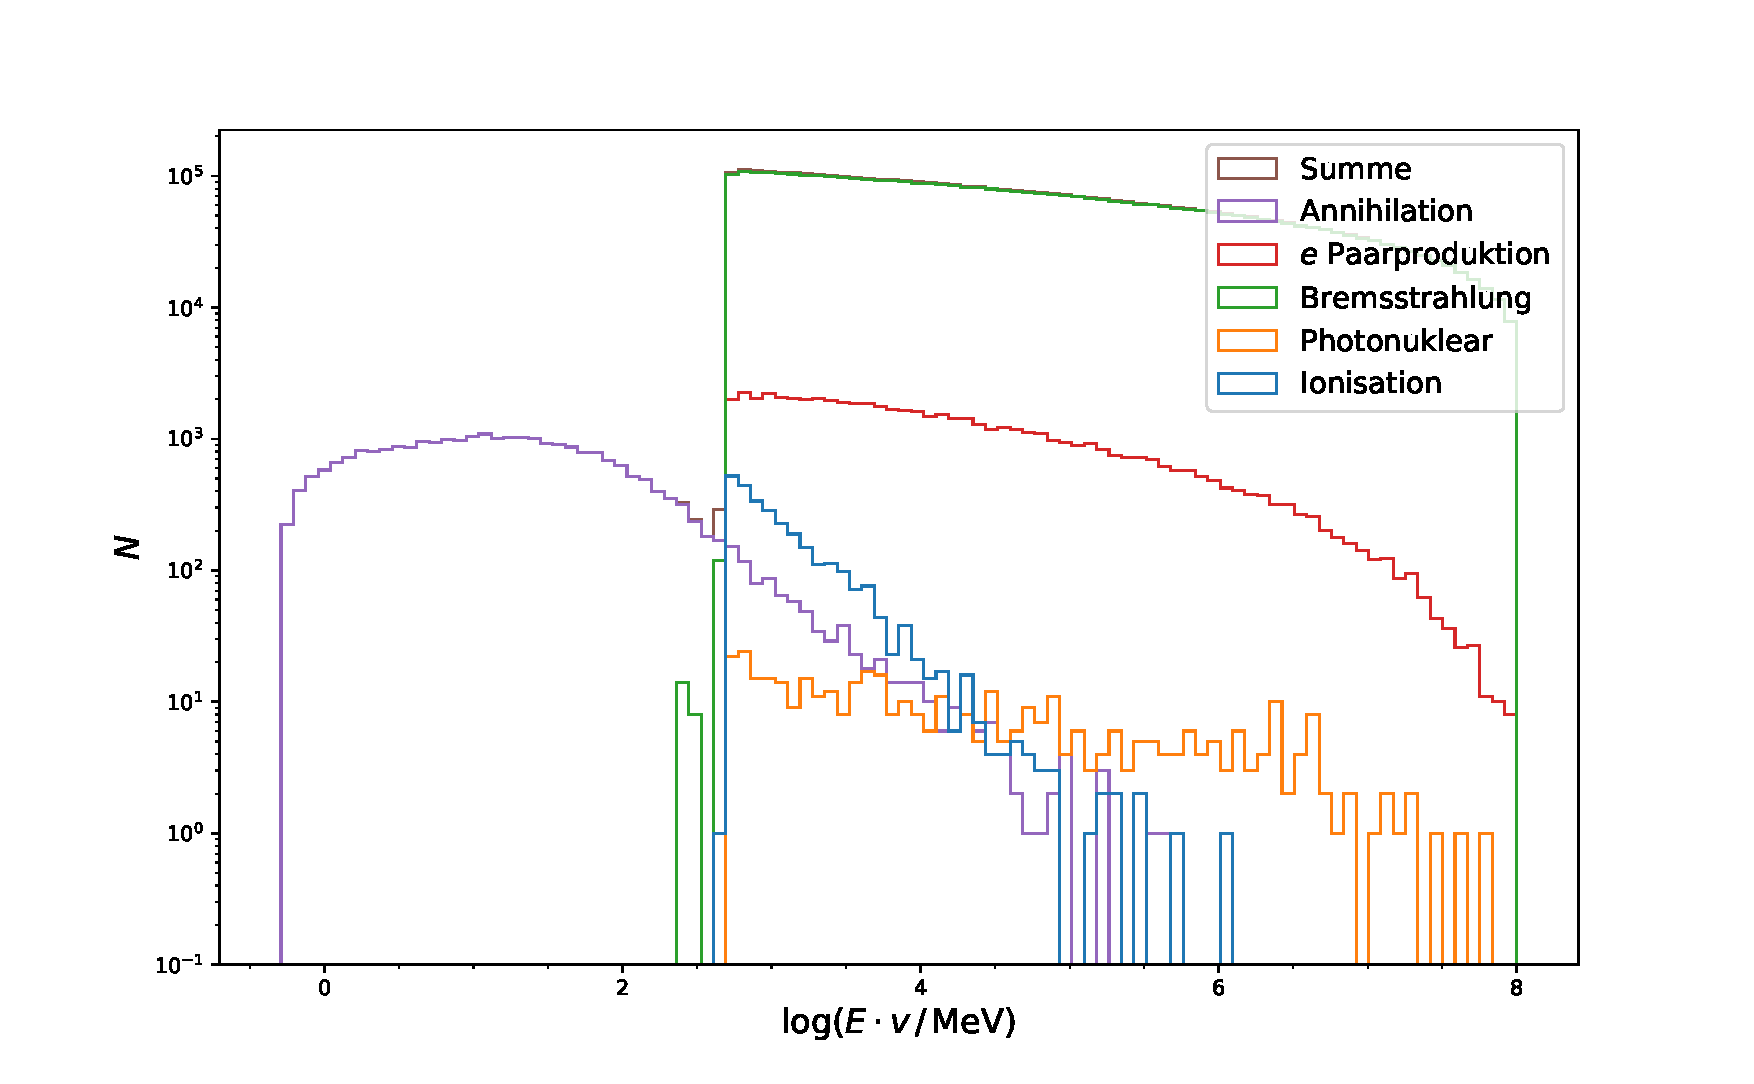
\includegraphics[height=0.9\textheight, trim=0.5cm 0.5cm 0.4cm 2cm,clip=true]{{plots/annihilation/all_standardrock_stats_100000_Emin_8.0_Emax_8.0_index_1}.pdf}
      \caption*{Energieverluste von $\num{e5}$ $e^+$ einer Startenergie von $\SI{e8}{\mega\electronvolt}$ durch Gestein, $E_\text{cut} = \SI{500}{\mega\electronvolt}$.}
      \label{fig:1}
  \end{figure}
\end{frame}


%% Photopropagation

\section{Schauerpropagation - Photonpropagation}


\begin{frame}{Paarbildung}
  \begin{columns}

    \column{0.4\textwidth}
    \begin{center}
      \begin{tikzpicture}
      \centering
       % Sizes
       \pgfmathsetmacro{\len}{0.05cm}
       \pgfmathsetmacro{\halflen}{\len/4}
       \pgfmathsetmacro{\vertexsize}{\len/20}
       \begin{feynman}
           % vertices
           \vertex (c) at (0, 0);
           \vertex (b) at (0, -1.5*\len);
           \vertex (f) at (-1*\len, -2*\len);
           \vertex (a) at (+1*\len, -2*\len);
           \vertex (e) at (-1*\len, 0.5*\len);
           \vertex (d) at (+1*\len, 0.5*\len);
     
           % draw diagram
           \diagram* {
             (a) -- [fermion] (b) -- [fermion] (c) -- [fermion] (d),
             (c) -- [boson] (e),
             (b) -- [boson] (f)
           };

           % labels
           \node[above] at (e) {$\gamma$};
           \node[below] at (f) {$\gamma_\text{Kern}$};

           \node[above] at (d) {$e^+$};
           \node[below] at (a) {$e^-$};
      \end{feynman}
    \end{tikzpicture}
  \end{center}

  \column{0.6\textwidth}
    \begin{itemize}
      \item Dominierender Prozess für hohe Energien
      \item Rein stochastische Wechselwirkung
      \item Analytische, approximative Formel für Wirkungsquerschnitt\footnotemark
      \item Verschiedene Modelle zur Bestimmung der Ablenkungswinkel der erzeugten Leptonen
      \begin{itemize}
        \item[$\rightarrow$] Effekte durch Ablenkung meist vernachlässigbar
      \end{itemize}
    \end{itemize}
  \end{columns}
  \footnotetext{Yung-Su Tsai, Pair production and bremsstrahlung of charged leptons}
\end{frame}



\begin{frame}{Comptonstreuung}
  \begin{columns}

    \column{0.4\textwidth}
    \begin{center}
      \begin{tikzpicture}
      \centering
       % Sizes
       \pgfmathsetmacro{\len}{0.05cm}
       \pgfmathsetmacro{\halflen}{\len/4}
       \pgfmathsetmacro{\vertexsize}{\len/20}
       \begin{feynman}
           % vertices
           \vertex (a) at (0, 0);
           \vertex (b) at (1.5*\len, 0);
           \vertex (c) at (-0.5*\len, 0.75*\len);
           \vertex (d) at (2*\len, 0.75*\len);
           \vertex (e) at (-0.5*\len, -0.75*\len);
           \vertex (f) at (2*\len, -0.75*\len);
     
           % draw diagram
           \diagram* {
             (e) -- [fermion] (a) -- [fermion] (b) -- [fermion] (f),
             (c) -- [boson] (a),
             (b) -- [boson] (d)
           };

           % labels
           \node[left] at (c) {$\gamma$};
           \node[right] at (d) {$\gamma$};

           \node[left] at (e) {$e^-$};
           \node[right] at (f) {$e^-$};
      \end{feynman}
    \end{tikzpicture}
  \end{center}

  \column{0.6\textwidth}
    \begin{itemize}
      \item Dominierender Prozess für niedrige Energien
      \item Wirkungsquerschnitt durch Klein-Nishina-Formel gegeben
      \item Ablenkungswinkel eindeutig durch Energien bestimmt
    \end{itemize}
  \end{columns}
\end{frame}


\begin{frame}
  \begin{figure}
      \centering
      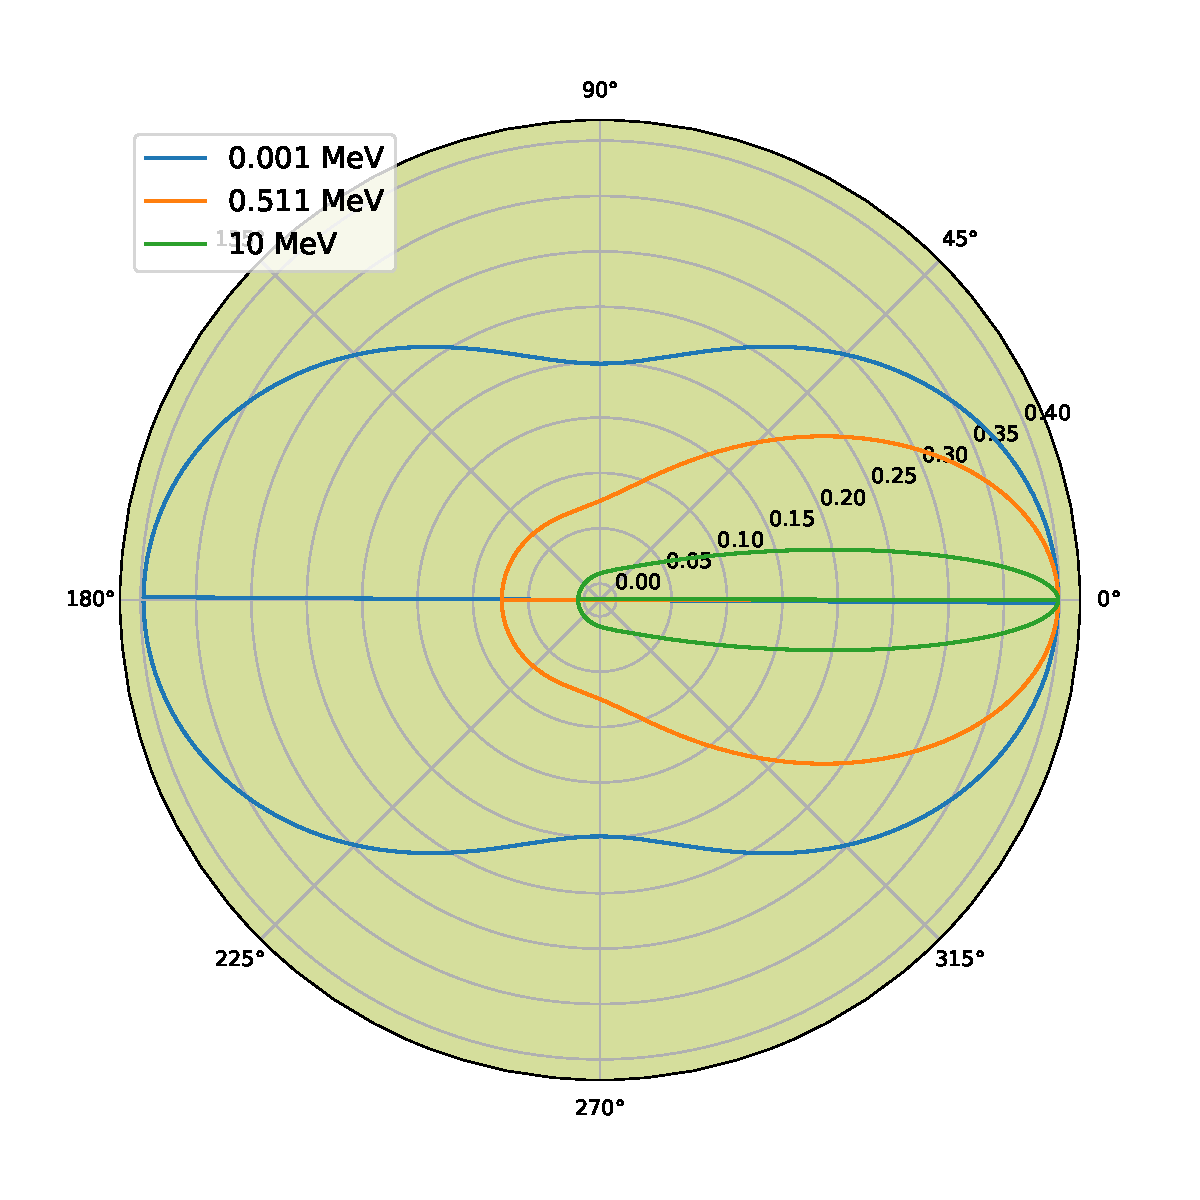
\includegraphics[height=0.8\textheight, trim=0.5cm 0.5cm 0.4cm 2cm,clip=true]{{plots/compton/compton}.pdf}
      \caption*{Klein-Nishina-Formel, differentiell in $\cos\left( \theta \right)$. Die radiale Achse zeigt den differentiellen Wirkungsquerschnitt in arbiträren Einheiten.}
      \label{fig:1}
  \end{figure}
\end{frame}


\begin{frame}
  \begin{figure}
      \centering
      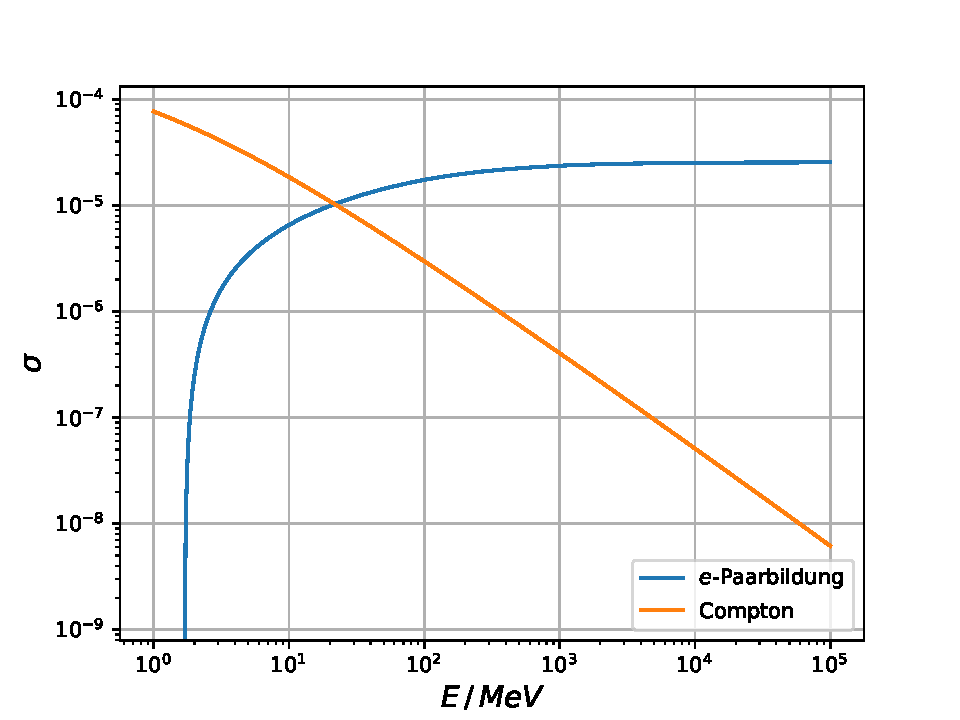
\includegraphics[height=0.9\textheight, trim=0cm 0cm 0.0cm 1.2cm,clip=true]{{plots/compton/compton_comparison_air}.pdf}
      \caption*{Vergleich der totalen Wirkungsquerschnitte für Photonen in Luft.}
      \label{fig:1}
  \end{figure}
\end{frame}


\begin{frame}
  \begin{columns}
    \column{0.55\textwidth}
      Mittlere freie Weglänge $\overline{\ell}$ für hochenergetische Photonen gegeben durch
        \begin{align*}
            \overline{\ell} \approx \frac{9}{7} X_0
        \end{align*}
      mit der Strahlungslänge in Luft: $X_0 \approx \SI{36.62}{\gram\per\square\centi\metre}$
  \column{0.45\textwidth}
      \begin{figure}
          \centering
          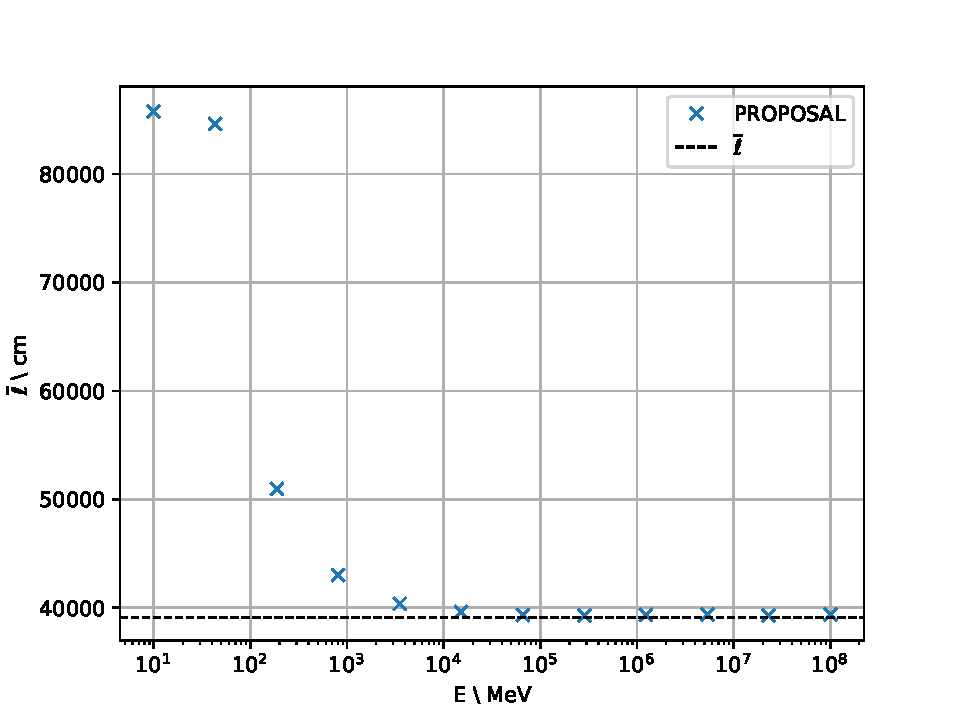
\includegraphics[height=0.65\textheight, trim=0cm 0cm 0.0cm 1.2cm,clip=true]{{plots/rad_length/rad_length}.pdf}
          \caption*{Reichweite von Photonen in Luft}
          \label{fig:1}
      \end{figure}
  \end{columns}
\end{frame}

%%% 4. Ergebnisse


\section{}

\begin{frame}[noframenumbering]{Inhalt}
   \begin{columns}
       \begin{column}{0.4\textwidth}

            \setbeamercolor{block title}{fg=white, bg=darkgray}
            \setbeamercolor{block body}{fg=darkgray, bg=gray}

            \begin{block}{1. Einführung in PROPOSAL}
              \centering
                \vspace{2mm}
              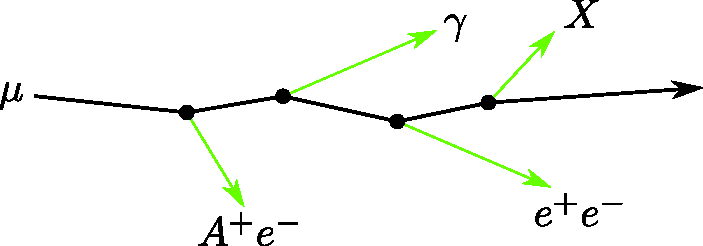
\includegraphics[height=0.15\textheight]{plots/muon_path.pdf}
                \vspace{2mm}
            \end{block}
       \end{column}
       \begin{column}{0.4\textwidth}

            \setbeamercolor{block title}{fg=white, bg=darkgray}
            \setbeamercolor{block body}{fg=darkgray, bg=gray}

            \begin{block}{2. Seltene Prozesse}
            \centering
            \vspace{2mm}
      \resizebox{!}{0.15\textheight}{%
            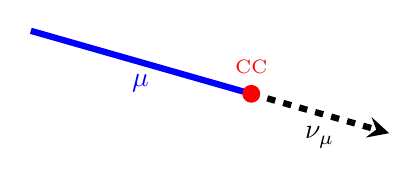
\begin{tikzpicture}
              \centering
                    
            \draw [line width=0.8mm, blue] (-1.9, 1.8) -- node[below] {$\mu$}  (0.9, 1.);     
            \draw [line width=0.8mm, black, dashed, ->, >=stealth] (0.9, 1.) -- node[below] {$\nu_{\mu}$}  (0.9+1.4+0.35, 1. - 0.4 - 0.1);      
            \draw[red,fill=red] (0.9, 1.) circle (0.7ex) node[label=above: $\scriptsize \text{CC}$]{};
          \end{tikzpicture}
        }
      \vspace{3mm}
            \end{block}
       \end{column}
   \end{columns}
   \begin{columns}
       \begin{column}{0.4\textwidth}

            \setbeamercolor{block title}{fg=white, bg=darkgray}
            \setbeamercolor{block body}{fg=darkgray, bg=gray}

            \begin{block}{3. Schauerpropagation}
            \centering
            \vspace{2mm}
      \resizebox{!}{0.15\textheight}{%

            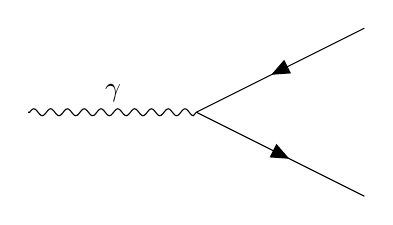
\begin{tikzpicture}
                  \centering
                   % Sizes
                   \pgfmathsetmacro{\len}{0.05cm}
                   \pgfmathsetmacro{\halflen}{\len/4}
                   \pgfmathsetmacro{\vertexsize}{\len/20}
                   \begin{feynman}
                       % vertices
                       \vertex (a) at (0, 0);
                       \vertex (b) at (1.5*\len, 0);
                       \vertex (c) at (3*\len, 0.75*\len);
                       \vertex (d) at (3*\len, -0.75*\len);;
                 
                       % draw diagram
                       \diagram* {
                         (c) -- [fermion] (b) -- [fermion] (d),
                         (a) -- [boson, edge label=\(\gamma\)] (b),
                       };   
                  \end{feynman}
            \end{tikzpicture}
            }
            \vspace{2.5mm}
           \end{block}
       \end{column}
       \begin{column}{0.4\textwidth}

            \setbeamercolor{block title}{fg=white, bg=tugreen}
            \setbeamercolor{block body}{fg=darkgray, bg=tulight}

           \begin{block}{4. Ergebnisse}
              \centering
                \vspace{2mm}
              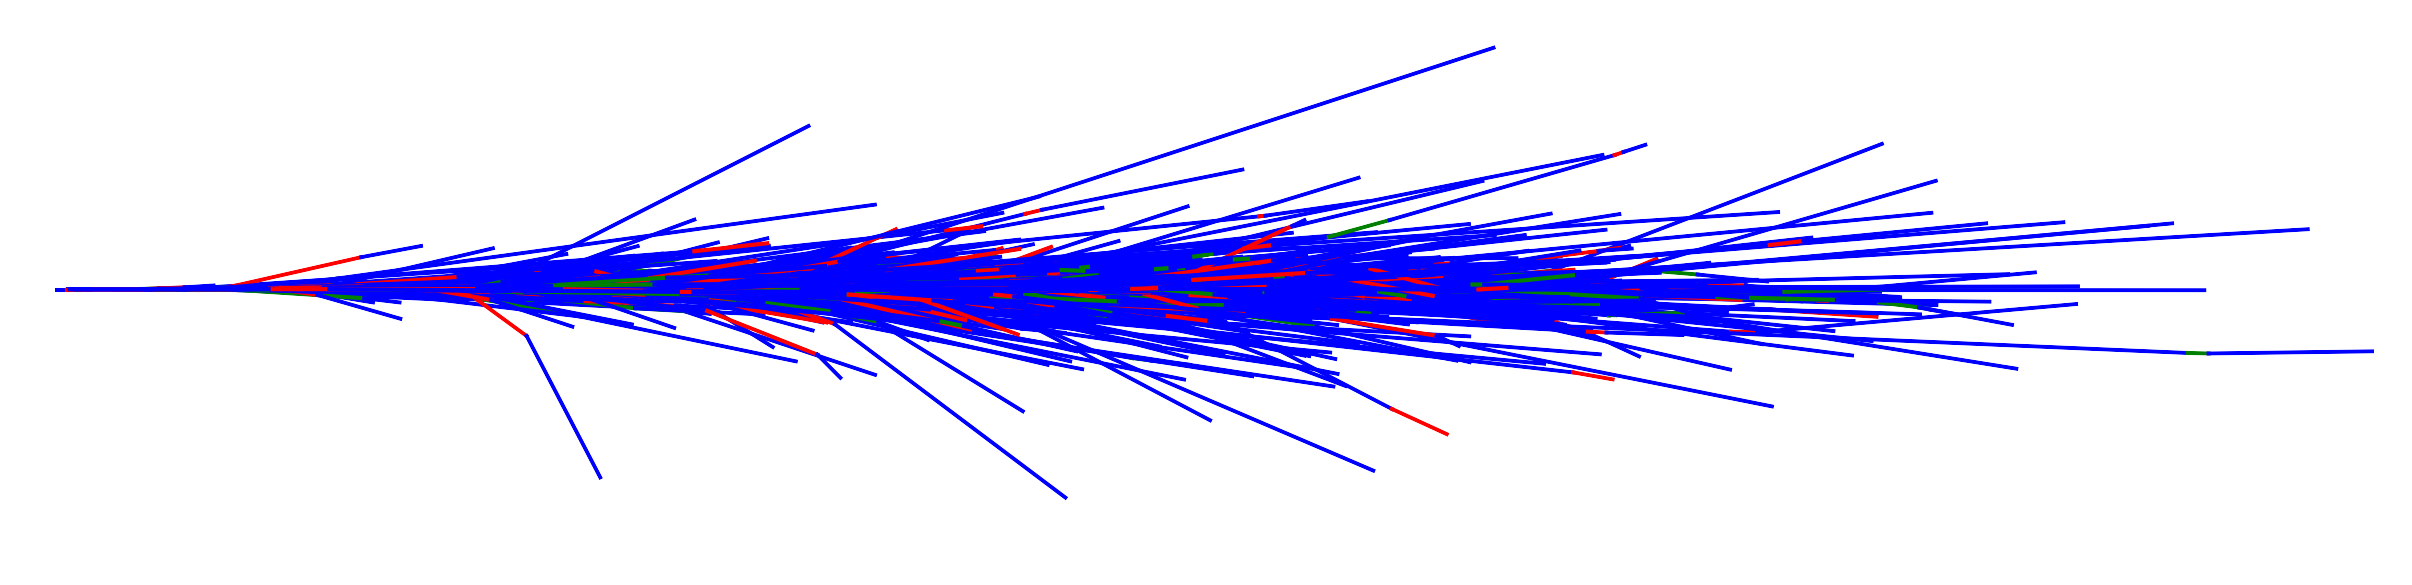
\includegraphics[height=0.15\textheight]{plots/shower_nolegend.png}
                \vspace{2mm}
           \end{block}
       \end{column}
   \end{columns}
\end{frame}


\section{Ergebnisse}

\begin{frame}{Erstellung eines Teilchenschauers}
\begin{center}
\begin{minipage}{0.7\textwidth}
\begin{figure}
\begin{algorithm}[H] %or another one check
\DontPrintSemicolon
     \SetAlgoLined
    Teilchenliste = [Primärteilchen]\;
     \While{Teilchenliste nicht leer}{
      Entnehme erstes Teilchen aus Teilchenliste\;
      Propagiere Teilchen\;
      Füge alle Sekundärteilchen der Teilchenliste hinzu\;
     }

\end{algorithm}
\caption*{Vereinfachter Algorithmus zur Schauerpropagation in \textbf{PROPOSAL}.}
\end{figure}
\end{minipage}
\end{center}
\end{frame}


\begin{frame}
   \vspace{-5mm}
  \begin{columns}
    \begin{column}{0.33\textwidth}
      \begin{figure}
          \centering
          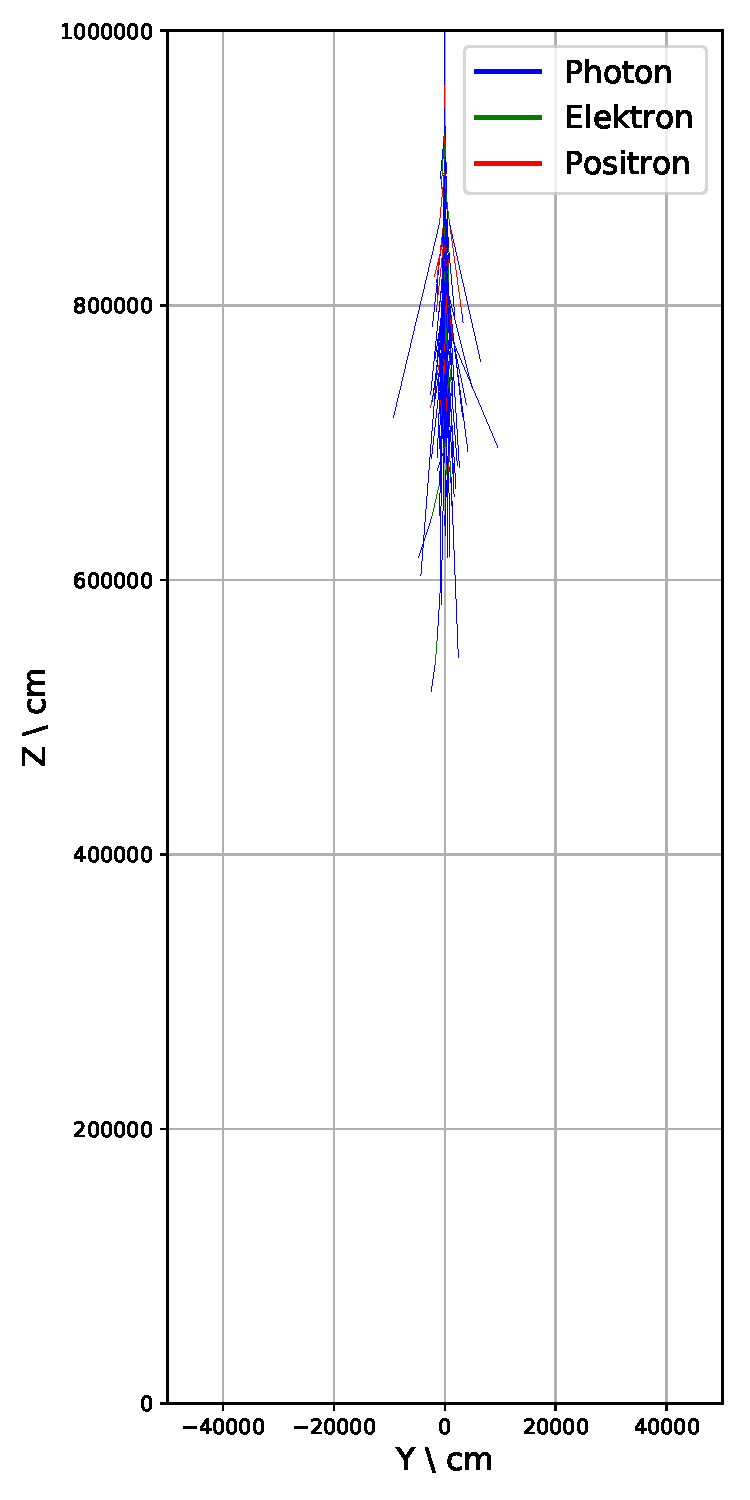
\includegraphics[height=0.9\textheight]{shower_presentation/2d_shower_1e5.pdf}
          \caption*{$E = \SI{e5}{\mega\electronvolt}$}
      \end{figure}
    \end{column}


    \begin{column}{0.33\textwidth}
      \begin{figure}
          \centering
          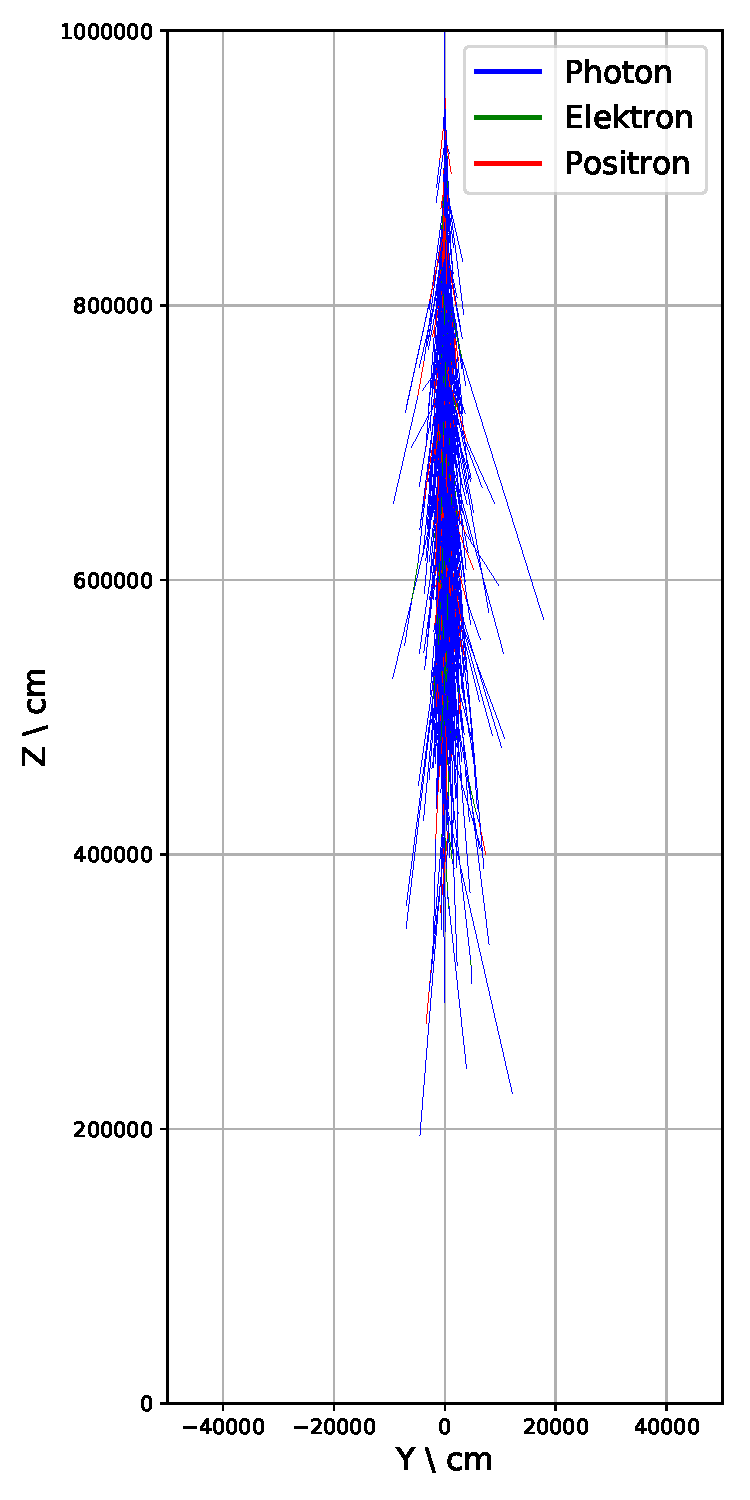
\includegraphics[height=0.9\textheight]{shower_presentation/2d_shower_1e6.pdf}
          \caption*{$E = \SI{e6}{\mega\electronvolt}$}
      \end{figure}
    \end{column}

    \begin{column}{0.33\textwidth}
      \begin{figure}
          \centering
          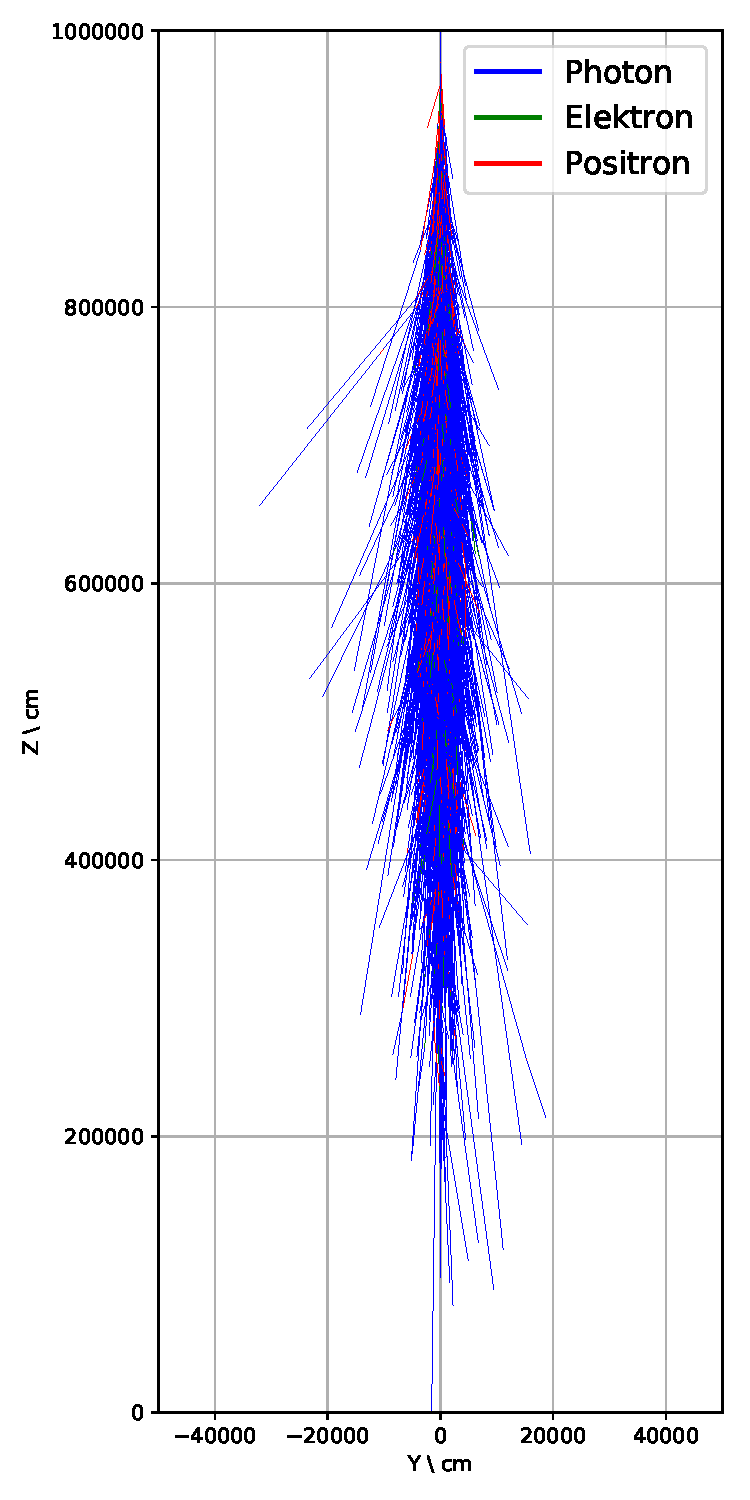
\includegraphics[height=0.9\textheight]{shower_presentation/2d_shower_1e7.pdf}
          \caption*{$E = \SI{e7}{\mega\electronvolt}$}
      \end{figure}    \end{column}
  \end{columns}
\end{frame}


\begin{frame}
   \vspace{-3mm}
  \begin{columns}
    \begin{column}{0.5\textwidth}
      \begin{figure}
          \centering
          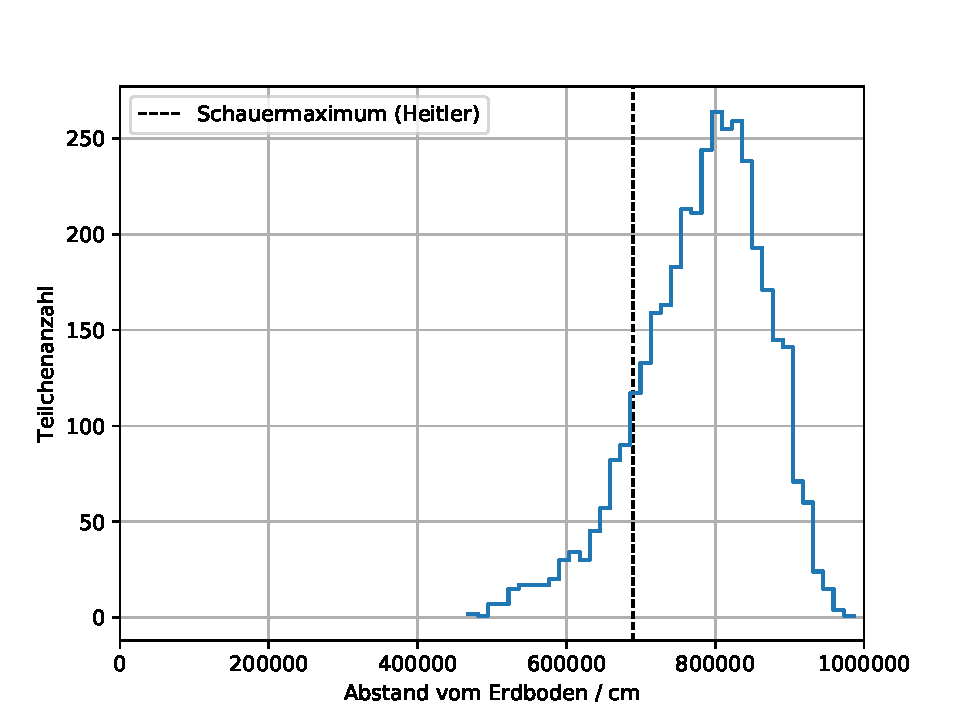
\includegraphics[height=0.7\textheight]{shower_presentation/hist_1e5.pdf}
          \caption*{$E = \SI{e6}{\mega\electronvolt}$}
      \end{figure}
    \end{column}

    \begin{column}{0.5\textwidth}
      \begin{figure}
          \centering
          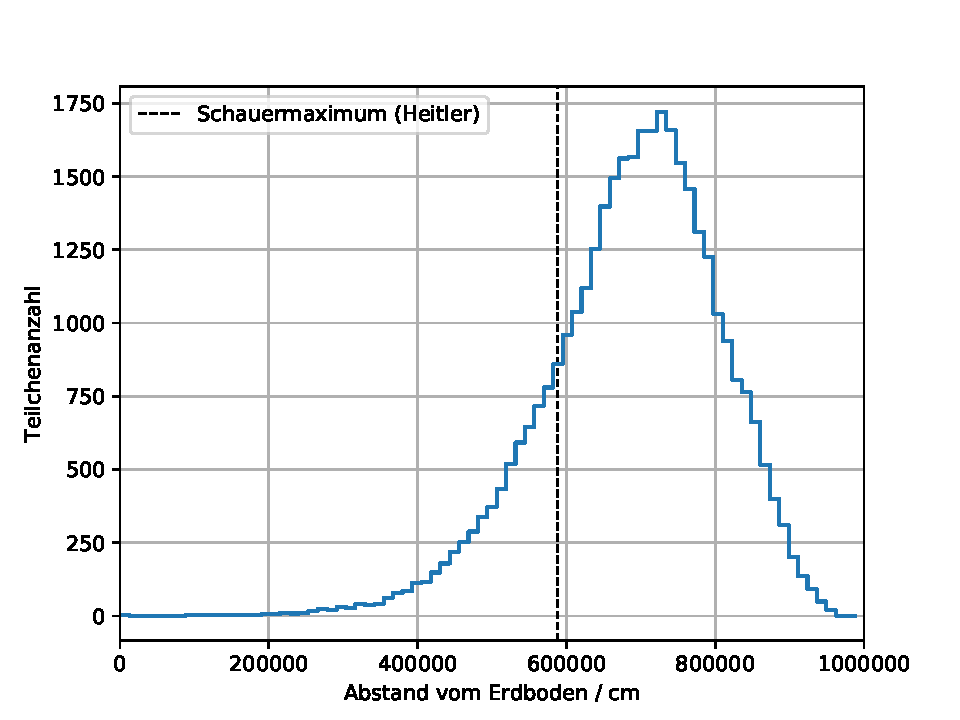
\includegraphics[height=0.7\textheight]{shower_presentation/hist_1e6.pdf}
          \caption*{$E = \SI{e7}{\mega\electronvolt}$}
      \end{figure}    
    \end{column}
  \end{columns}
  \begin{figure}
  \caption*{Teilchenanzahl gegen die Schauertiefe, verglichen mit dem erwarteten Schauermaximum im Heitler-Schauer-Modell.}
  \end{figure}
\end{frame}

%%% End

\section{Zusammenfassung und Ausblick}

\begin{frame}{Zusammenfassung}
    \textbf{Seltene Prozesse}
   \begin{itemize}
    \setlength\itemsep{0.5em}
    \item Myonpaarproduktion als neuer Prozess verfügbar 
    \item Schwache Wechselwirkung als neuer Prozess verfügbar
   \end{itemize}

   \textbf{Schauerpropagation}
   \begin{itemize}
    \setlength\itemsep{0.5em}
    \item Überarbeitere Wechselwirkungen für $e^+/e^-$
    \item Annihilation als neuer Prozess für $e^+$
    \item Paarbildung und Comptonstreuung als Prozesse für Photonen
    \item[$\Rightarrow$] Propagation elektromagnetischer Schauer in PROPOSAL prinzipiell möglich
   \end{itemize}
\end{frame}


\begin{frame}{Ausblick}
    \textbf{Seltene Prozesse}
   \begin{itemize}
    \setlength\itemsep{0.5em}
    \item Explizite Simulationen nötig um die Relevanz der neuen Prozesse überprüfen zu können
   \end{itemize}

   \textbf{Schauerpropagation}
   \begin{itemize}
    \setlength\itemsep{0.5em}
    \item Untersuche Schauerpropagation in inhomogenen Medien (realistische Atmosphäre)
    \item Einbindung von \textbf{PROPOSAL} in \textbf{CORSIKA}
    \item[$\rightarrow$] Komplette Schauerpropagation
    \item[$\rightarrow$] Vergleiche mit anderen physikalischen Modellen (z.B. EGS5, EmCa)
   \end{itemize}
\end{frame}


\begin{frame}[t]
  \vspace{-5mm}
  \begin{minipage}[t][0.8\textheight][t]{\textwidth}
      \begin{columns}
    \column{0.5\textwidth}
      \begin{figure}
          \centering
          
\includegraphics[width=0.6\linewidth]{plots/github.pdf}
           \captionsetup{format=myformat}
          \caption*{https://github.com/tudo-\\astroparticlephysics/PROPOSAL}
      \end{figure}
    \column{0.5\textwidth}
      \begin{figure}
          \centering
          
\includegraphics[width=0.6\linewidth]{plots/arxiv.pdf}
          \captionsetup{format=myformat}
          \caption*{https://arxiv.org/abs/1809.07740 \\ \phantom{astroparticlephysics/PROPOSAL}}
      \end{figure}
  \end{columns}
  \end{minipage}
  \vfill
  \begin{minipage}{\textwidth}
      \smaller
      \begin{center}
      PROPOSAL may be modified and distrubuted under terms of a modified LGPL license.\\More information on our GitHub page.
      \end{center}
  \end{minipage}
\end{frame}
\end{document}
